%% GENERATED FILE -- do not edit.
%% Built by our_papers/paper1_variance_aware/latex/build_paper.py from the Markdown drafts in ../draft
%% Edit the draft, then re-run:  python our_papers/paper1_variance_aware/latex/build_paper.py
%%
%% SELF-CONTAINED: the layout is inlined below rather than pulled from a .sty, so this file plus
%% refs.bib and figures/ is the whole project. One less thing to forget when uploading.
%%
%% This is the NAMED reading copy. The journal submission (Expert Systems with Applications) is the
%% anonymised build that build_paper.py writes to ../eswa_submission/manuscript/ on elsarticle.
\documentclass[10pt]{article}

%% ---- inlined layout (the ESWA build swaps it for elsarticle) ----------------------------------
%% Set to roughly the density a single-column ML venue typesets at. The first version of this
%% block was loose -- 11pt, extra leading, a blank line between every paragraph -- and cost about
%% seven pages of nothing. Layout is not content; do not solve a length problem by cutting text
%% until the layout is honest.
\usepackage[letterpaper,margin=1in]{geometry}
\usepackage{times}
\usepackage{titlesec}
\newcommand{\name}{}
\newcommand{\email}{\quad\texttt}
\newcommand{\addr}{}
\newcommand{\AND}{\\[0.6em]}
\setlength{\parskip}{0pt}
\setlength{\parindent}{1.2em}
\titleformat{\section}{\normalfont\large\bfseries}{\thesection}{0.6em}{}
\titleformat{\subsection}{\normalfont\normalsize\bfseries}{\thesubsection}{0.6em}{}
\titlespacing*{\section}{0pt}{1.1em}{0.35em}
\titlespacing*{\subsection}{0pt}{0.8em}{0.25em}
\setlength{\textfloatsep}{10pt plus 2pt minus 2pt}
\setlength{\intextsep}{10pt plus 2pt minus 2pt}
\setlength{\abovecaptionskip}{4pt}
%% --------------------------------------------------------------------------------------------

\usepackage{graphicx}
%% Look for figures both in figures/ and beside the .tex, so the document still finds them if the
%% upload flattens the folder -- the commonest way this breaks on a fresh Overleaf project.
\graphicspath{{figures/}{././}}
\DeclareGraphicsExtensions{.pdf,.png}
\usepackage{array}
\usepackage{booktabs}
\setlength{\tabcolsep}{4pt}
\renewcommand{\arraystretch}{0.95}
\usepackage[inline]{enumitem}
\setlist{nosep,leftmargin=1.5em,topsep=2pt}
\usepackage{amsmath,amssymb}
%% Text-layer extraction. Computer Modern math has no ToUnicode CMap, so every $\sigma$ in
%% this paper renders correctly and copies out as nothing -- which is how three separate
%% reviews came to report symbols as 'missing' from a file that contains no non-ASCII
%% character at all. cmap must load BEFORE fontenc. It changes no pixel of the output.
\usepackage{cmap}
%% pdfLaTeX-only primitive, guarded so the same file also compiles under XeTeX (build_pdfs.py).
\ifdefined\pdfgentounicode\input{glyphtounicode}\pdfgentounicode=1\fi
\usepackage[utf8]{inputenc}
\usepackage[T1]{fontenc}
\usepackage{microtype}
\usepackage[colorlinks=true,allcolors=blue]{hyperref}
\usepackage{natbib}
\usepackage{caption}
\captionsetup[table]{skip=4pt}

\title{Ablation Tables as Measuring Instruments:\\ Run-to-Run Variability, Confounds and a Positive Control
in Infrared--Visible Image Fusion}

%% Author list. Order chosen by the authors: the student who performed the work first, the
%% principal supervisor last -- the senior-author-last convention, standard in ML venues.
%% Titles stay out of the \name line (no venue prints them there); the position goes in the
%% affiliation, as the authors supplied it on 2026-09-14. Supervisory roles are not printed in a paper.
%% 2026-10-25: Prof. El-Mikaty replaces Prof. Amer, on the author's instruction after the supervision
%% committee was re-registered. His \email is deliberately LEFT OUT -- the address is not yet
%% available and MUST be added before submission. (An empty \email does not compile: the local
%% stub's \email takes an argument and swallowed the \\.)
\author{\name Mostafa Moawad Mostafa Nada \email mostafa.nada1282@gmail.com \\
        \addr MSc Researcher, Electronics and Communications Engineering Department \\
              Faculty of Engineering, Mansoura University, Egypt
        \AND
        \name Abdelgwad Elashry \email A.elashry@gaf.edu.eg \\
        \addr School of Engineering and Computer Science \\
              University of Hertfordshire hosted by GAF, Egypt
        \AND
        \name Hamdy Ahmed Ahmed El-Mikaty \\
        \addr Emeritus Professor, Electronics and Communications Engineering Department \\
              Faculty of Engineering, Mansoura University, Egypt}

\begin{document}
\maketitle

\begin{abstract}
Design decisions in infrared--visible image fusion rest on ablation tables that report one training run per setting, with no estimate of run-to-run variability and no check that the metrics respond to a real change. We supply both, for two methods from unrelated families, across 239 training runs, and contribute an evaluation protocol assembled from established practice. Re-measured at eight seeds per setting, a complete ablation yields \textbf{one of 27 comparisons significant uncorrected and none after correction for multiplicity}; that cell does not replicate, and the published ranking is not reproduced. A second test set separates the same checkpoints only by about one $\sigma$. CrossFuse's Top-K ablation also removes 47 \% of the training data; with volume held fixed, the mechanism shows no detected effect. A parameter-randomisation control on both architectures shows that responsiveness is a property of the metric and the network: on the first, two of nine metrics did not separate a random-weight network from a trained one after correction, even at twenty seeds; on the second, two others rank the untrained network \emph{above} the trained one, because its decoder returns the visible input. Finally, weight tying makes depth independent of parameter count: at the published depth the 2.46$\times$ smaller model differs from the original on no metric after correction, and at depth 8, in registered tests on new seeds, it leads its untied counterpart on four metrics and the published configuration on RoadScene and MSRS, trading contrast for fidelity on TNO.
\end{abstract}
\noindent\textbf{Keywords:} Infrared and visible image fusion; Ablation study; Run-to-run variability; Positive control; Fusion quality metrics; Reproducibility.

\section{Introduction}

An ablation table operates as an empirical measuring instrument whose precision must be characterised before its readings are interpreted. Validating such tables requires establishing two baselines: the metric noise floor under repeated retraining (seed and hardware non-determinism together), and a positive control demonstrating metric responsiveness to known model degradations. At the costs measured in this study \,---\, about one GPU-hour per seed on LRRNet and three on CrossFuse \,---\, neither is expensive. In machine learning generally, the first is established practice \citep{henderson,bouthillier,pineau,colas} and the second exists in at least one subfield \citep{adebayo}.

This paper asks what happens when both are supplied to a literature that reports neither. The testbed is infrared--visible image fusion (IVIF), chosen because it has the properties that make the question sharp: no ground truth, so quality is reported through a battery of nine surrogate metrics; architectures from unrelated families in active competition; and ablation tables, in every paper we examined, consisting of single training runs with no variance estimate.

\textbf{This study does not assess the merit of the two methods.} Two published methods are re-measured because a defect must be demonstrated on something, and they were selected by measured cost rather than by argument. The claim is about what a table of that construction can demonstrate \,---\, never about the competence or good faith of anyone who published one. Where the measurements favour those papers, they are reported with the same prominence as where they do not, and the reader will find several places where they do.

\subsection{Questions}

\begin{enumerate}
\item \textbf{What is $\sigma$} \,---\, the spread of each metric when identical code is retrained with a different seed?
\item \textbf{Read against $\sigma$, do published ablation tables support the conclusions drawn from them?}
\item \textbf{Can the metrics detect a difference at all}, and what is the smallest one they resolve?
\item \textbf{Can an architecture be designed so that the confound cannot be constructed}, rather than controlled for after the fact?
\end{enumerate}

\subsection{Contributions}

This work does not introduce a new statistical test. It contributes an evaluation protocol for ablation studies in IVIF, assembled from established practice, and demonstrates on two architectural families how run-to-run variability, capacity confounds and architecture-dependent metric responsiveness change what a single-run ablation table can show.

\begin{enumerate}
\item \textbf{$\sigma$ measured for two architecture families}, at three to twenty seeds. We have found no prior IVIF work that reports it. A by-product measured on both: two runs at the \emph{same} seed, same code and same container, differ by up to \textbf{44 \% of $\sigma$ on one architecture and 257 \% on the other} (the larger of two pairs, against a $\sigma$ from three seeds; 229 \% and 310 \% in two later pairs, against a $\sigma$ from five seeds; each is the largest same-seed difference across the nine metrics as a share of that arm's seed-to-seed $\sigma$, a measure of run-to-run noise rather than of fusion quality; Section~3). On the second, same-seed runs differ almost as much as runs at different seeds \,---\, recording it is necessary but not sufficient for reproducibility unless deterministic algorithms are enforced, which on LRRNet made same-seed runs bit-identical at a 20 \% time cost.
\item \textbf{A published ablation table re-measured entire} \,---\, all four settings retrained here, one evaluator, $\sigma$ from those same runs, eight seeds per setting. \textbf{One of 27 comparisons reaches significance uncorrected, and none survives a Holm or permutation max-\emph{t} correction} \,---\, and the published \emph{ordering} is not reproduced either. Twenty-three of the 27 differences are equivalent within $\pm$1.75 $\sigma$, the resolution the run's power analysis registered (an equivalence test chosen after the run; the follow-up registered it in advance); the other four were inconclusive, and a registered follow-up at twenty seeds found all four equivalent \,---\, while the one significant cell did not replicate. At three seeds the count was zero; the run that raised it was registered, with the reading that would withdraw that headline, before it began. \textbf{On a second test set} (RoadScene), the same checkpoints re-scored without retraining separate \textbf{four of 27 after correction} (within each nine-metric comparison) \,---\, each about 1 $\sigma$, ordering the settings 2 > 4 > 6; on TNO the same ordering appears only before correction (8 of 18 comparisons at twenty seeds), and on neither set is the published choice of 4 supported as best.
\item \textbf{A positive control, adopted rather than invented.} Applying the parameter-randomisation test of \citet{adebayo} to fusion metrics on \textbf{both} architectures, five seeds per arm. \textbf{SF and AG did not separate random weights from a fully trained LRRNet after correction, even at twenty seeds per arm} (each nominally significant, p $\approx$ 0.03); on the second architecture they are the \emph{strongest} detectors of the nine, and \textbf{MI and VIF instead rank the untrained network above the trained one} \,---\, because its decoder returns the visible input, and they reward that; CDDFuse's released model, whose decoder CrossFuse inherits, is outranked by the same copy \,---\, one decoder lineage, whose two untrained networks share their weights, not two independent designs. A released method outside that decoder lineage, SeAFusion, provides a contrasting result: its untrained output does not copy the visible input (r = $-$0.12), and MI and VIF rank it far below the released model. Whether a measure responds is a property of the measure and the network together, so \textbf{a control cannot be assumed to carry over \,---\, on the two architectures measured here it did not, and each architecture--metric pair needs its own}. The milder arm, half the training budget, was repeated on the second architecture too and changed its answer in the same way: \textbf{2 of 9 resolve it there after correction (a third, Q$^{AB/F}$, only uncorrected) against 0 of 9 on the first, and the two that do are the two that invert.} It shows that 7 of the 9 metrics respond to gross failure on the architecture the nulls were measured on; it does not show sensitivity at the effect sizes an ablation probes, so the nulls are read only at their stated resolution, through equivalence tests.
\item \textbf{Parameter-count matching by construction.} Weight-tied unrolling makes the parameter count constant in depth, giving a \textbf{2.46$\times$ smaller} model with no metric differing after correction under the published training budget \,---\, where the metrics stop registering further training by the second of four epochs, and twice the budget improves none of them on either network (Section~6) \,---\, and a depth ablation in which the confound cannot be built: at constant size, eight solver iterations against four move 0 of 9 metrics and seven are shown equivalent. Across the resulting 2$\times$2 at five tied seeds, 5 of 36 comparisons cross uncorrected, all favouring the tied model and none surviving correction \,---\, and a registered test on twelve new seeds per arm then confirmed the one contrast they concentrated in: \textbf{at depth 8 the tied network beats the untied one on all four metrics after correction, on two test sets} (three of the four on a third), and, 2.46$\times$ smaller than the published configuration, is better than it on RoadScene and MSRS with no metric against, while on TNO it trades SD for VIF, Q$^{AB/F}$ and SSIM \,---\, the outcome a registered test on further new seeds, against baseline seeds outside every earlier comparison, returned.
\item \textbf{A volume-controlled test of a published mechanism}, which the original design cannot perform because it varies corpus size and mechanism together. The larger run-to-run spread we measured when retraining its ablation without the mechanism (median 2.17$\times$, not tested for significance) cannot be attributed to the mechanism: held at constant corpus size, no effect of the mechanism itself is detected, at eight seeds per arm on the second architecture and at five per arm on CrossFuse itself, where whether that larger spread comes from the mechanism or from the lost data remains unresolved at that sample size.
\item \textbf{Two documented cases in which published IVIF metric values are not commensurable across papers}, so printed tables cannot safely be compared without the evaluator.
\end{enumerate}

\subsection{What is not claimed}

No general improvement in fusion quality is claimed. Two of the three modifications tested produced nulls, and they are reported at the same length as the one that did not. The efficiency result is categorical: a parameter count has no run-to-run variability. The one quality result is scoped by metric and test set: against the published configuration, the weight-tied network at depth 8 is better on several metrics on RoadScene and MSRS and trades SD for fidelity on TNO, in registered tests on new seeds and on a substitute training corpus (Section~3).

The same protocol was applied to our own claims, and those it withdrew or corrected are recorded in Section~3 rather than deleted. Two are worth naming here: this paper stated a limitation, named the two experiments that would settle it, ran both, and both cost a claim its generality, in the same direction each time.

\subsection{Structure}

Section~2 places the work against IVIF evaluation research and the variance literature. Section~3 states the protocol. Section~4 and Section~5 apply it to two published methods. Section~6 asks whether the confound can be designed away. Section~7 supplies the positive control that licenses the nulls. Section~8 discusses what follows for how the field ablates, and Section~9 states the limits.

\section{Related work}

\subsection{Infrared--visible image fusion}

Deep IVIF has converged on two broad families. The first decomposes features into complementary streams and processes each with a different operator: CDDFuse \citep{cddfuse} splits low- and high-frequency content between a Restormer-derived attention block \citep{restormer} and an invertible CNN, a design inherited with a new data recipe by CrossFuse \citep{crossfuse-shi}, and extended by a substantial subsequent literature \citep{ddfm,emma,text-if}. The second builds the network by unrolling a classical optimisation procedure, so that each layer corresponds to one iteration of a solver: LRRNet \citep{lrrnet} unrolls a low-rank-and-sparse decomposition in the manner of LISTA \citep{lista}, following the same group's earlier designs \citep{densefuse,nestfuse,rfn-nest,res2netfuse}, and has itself been extended in several directions \citep{grformer,ferfusion}. This paper takes one method from each family, so that we can test whether an observed phenomenon persists across two distinct architectural families rather than being specific to one architecture.

\subsection{Evaluating fusion}

Because IVIF has no ground truth, quality is reported through a standard battery of no-reference and source-referenced measures \,---\, SSIM \citep{ssim}, VIF \citep{vif}, Q$^{AB/F}$ \citep{qabf}, SCD \citep{scd}, and the information- and gradient-based statistics MI \citep{qu-mi}, EN \citep{roberts-en}, SD, SF \citep{eskicioglu-sf} and AG \citep{cui-ag}, surveyed in \citep{ivif-survey}. VIFB \citep{vifb} established a common benchmark for comparing methods under these measures. Outside fusion, eleven full-reference quality models have been compared as \emph{optimisation objectives} for four image-processing tasks and judged by subjective tests on what they produced, motivated by the risk that heavy reuse of the same perceptual databases overfits the measures \citep{ding-iqa}. Judging a measure by what it rewards, rather than only by its agreement on a database, is the shift Section~7 makes for MI and VIF.

The reliability of the measures themselves has recently become an active question. EvaNet \citep{evanet} proposes a consistency framework for IVIF assessment; EVAFusion \citep{mllm-ivif} contributes an expert-annotated benchmark of 9,350 fused images and applies multimodal language models to the scoring problem; and further work seeks to bridge automatic scores to human judgement directly \citep{human-ivif} or to learn a pairwise preference measure \citep{pairwise-ivif}. \textbf{EvaNet shares four authors with LRRNet itself}, whose ablation table this paper re-measures \,---\, the group is already working on the trustworthiness of fusion evaluation. The other three are from three \textbf{unrelated} groups. That distribution is itself informative: four independent teams arriving at the reliability of these measures is stronger evidence that the problem is real than one group revisiting its own work would be.

\textbf{That line of work and this one are orthogonal.} It asks whether a metric agrees with a human observer. This paper asks a question that is logically prior: whether a difference a metric reports is larger than the difference produced by retraining the same configuration with a different random seed. A metric perfectly aligned with human perception is still unusable in an ablation table if the effect it reports is smaller than that noise. We have found no IVIF work that measures it, in either the visible--infrared setting or the neighbouring multi-focus and medical fusion literatures, where ablations likewise vary loss terms and fusion rules but not seeds.

\textbf{A third response replaces the surrogate measures with a downstream task.} SeAFusion \citep{seafusion} places fusion in the loop of a semantic-segmentation network and judges fused images by what that network can do with them; TarDAL \citep{tardal} couples fusion to object detection and contributes a multi-scenario benchmark on which detection is the yardstick. Scoring a fused image by its use addresses the failure Section~7 documents directly: an output that erases a person from the scene should not help a detector find them, whatever its MI. It does not address the question this paper asks. A segmentation or detection score is itself the output of a trained model, with its own run-to-run spread, so a difference in it supports a conclusion only against that spread; and whether the downstream score responds to fusion quality at all is exactly what a positive control establishes. The protocol of Section~3 carries over to task-driven evaluation unchanged. \citet{guan-rethink} take the same route with a segmentation-oriented evaluation, and report that existing fusion methods perform comparably to, or worse than, the visible image alone \,---\, a finding reached through a downstream task that Section~7's copy of the visible image reaches through the metrics themselves.

\subsection{Variance and controls in machine learning}

Outside fusion, the consequences of ignoring run-to-run variation are documented. \citet{henderson} showed that published reinforcement-learning comparisons could be reversed by seed choice alone; \citet{colas} gave the power analysis relating the number of seeds to the effect a comparison can resolve; \citet{bouthillier} decomposed benchmark variance into its sources and argued that ignoring them inflates apparent progress; Picard \citep{picard} scanned up to $10^4$ seeds of standard vision architectures and found outliers far from the mean easy to obtain; and \citet{pineau} set out reproducibility practice for the field. Reporting a mean and standard deviation over several seeds is, in that literature, unremarkable.

A second and less common practice is the \emph{positive control}: an intervention whose effect is known in advance, used to establish that a measurement instrument responds at all. \citet{adebayo} introduced the parameter-randomisation test for saliency methods \,---\, compare a trained model against the same architecture with random weights, and a method that cannot distinguish them is not explaining the model. We adapt that control: its manipulation, randomised weights against trained ones, is kept, while the measure it is read through changes from a saliency map to the fusion \emph{metrics}. To our knowledge it has not been applied to image-quality measures, and the adjacent IQA robustness literature asks different questions, concerning adversarial attacks on learned quality models and generalisation across distortion types.

\subsection{What is absent}

Two things follow. Published IVIF ablation tables report single training runs with no variance estimate, so the precision of the instrument producing them is unknown; and no published control establishes that the metrics can resolve a difference at all, so a reported ``no change'' cannot be distinguished from a metric that does not respond. This paper supplies both, for two methods from unrelated families, and reads the published tables against the result.

\textbf{Search scope.} The absence statements in this paper (no IVIF work found that reports run-to-run variance, or that runs a positive control on its metrics) rest on targeted searches made in September and October 2026: general web and arXiv searches combining infrared--visible image fusion with seed, run-to-run variance, multiple runs, standard deviation across runs, reproducibility, sanity check, randomly initialised network and positive control, together with the survey and benchmark lists cited in this section. The hits report SD as a quality metric, not as variation across runs. This is a targeted search, not a systematic review, and the statements are worded accordingly.

\section{Protocol}

Precision is used here operationally: the run-to-run variability of the whole train-and-evaluate pipeline, quantified per metric by the standard deviation $\sigma$ across retrainings. Four principles follow, each fixed before the results it governs existed.

\subsection{Measuring \texorpdfstring{$\sigma$}{sigma}}

The precision of interest is the spread produced by re-running the identical configuration and changing only the random seed. We train each reference configuration repeatedly under one code version, one corpus, one evaluator and one container image, varying nothing but the seed, and report the sample standard deviation $\sigma$ per metric. All training runs used Kaggle's NVIDIA Tesla T4 GPUs (16 GB) with PyTorch 2.10.0 built for CUDA 12.8; the CrossFuse checkpoint reproduction and the SeAFusion control ran on CPU with PyTorch 2.2.2. An AI assistant (Claude, Anthropic) was used throughout the research to write and revise the training-patch, evaluation, analysis and build scripts, to draft the registration files, and to check the reported numbers for consistency. Every training run was launched and its log checked by the authors, every registration was committed before its run, and every statistic reported here is recomputed from the recorded per-run metrics by separate audit scripts against which the authors checked each reported value.

Two properties of that measurement matter. First, \textbf{the released code of both methods seeds nothing} \,---\, LRRNet contains no seeding call at all, and randomness enters from two independent generators, so ``runs differing only in the seed'' was not an executable phrase until seeding was added. Second, \textbf{cudnn is deliberately left non-deterministic.} $\sigma$ must describe what a reader re-running the released code actually meets, and forcing determinism would understate it; a smaller $\sigma$ makes more published differences look real, which would weaken the very argument it supports. The cost of that choice is measurable, and it was measured on both architectures. Two runs at the \emph{same} seed, same code, same data and the same pinned container differ by up to \textbf{44 \% of $\sigma$ on LRRNet} (median 16 \%) and by up to \textbf{257 \% of $\sigma$ on CrossFuse} in the first measurement \,---\, two same-seed pairs from the half-budget arm, $\sigma$ from three seeds, the larger gap on SD \,---\, and by up to 229 \% and 310 \% in two later pairs from the $k = 0$ arm ($\sigma$ from five seeds, both on MI), declared as descriptive measurements before their numbers were read. Each CrossFuse figure is the largest absolute difference between the two runs' TNO means across the nine metrics, divided by the seed-to-seed sample $\sigma$ of the arm the pair belongs to; it measures run-to-run nondeterminism, not a change in fusion quality. GPU kernel selection was left nondeterministic in all of these runs; on LRRNet, enforcing deterministic algorithms made same-seed runs bit-identical, which identifies the source there, but this was not tested on CrossFuse. The CrossFuse figures are the more informative: averaged over the four pairs and nine metrics, same-seed runs differ by 0.88 $\sigma$ (median 0.55 $\sigma$), against about 1.13 $\sigma$ expected if the seed contributed nothing. Hardware nondeterminism is therefore a large part of the spread on CrossFuse, but four pairs, with $\sigma$ estimated from three to five seeds, cannot separate its share from the seed's. \textbf{Recording a seed is therefore necessary but not sufficient for reproducibility} at the precision an ablation table claims to resolve. The across-seed $\sigma$ estimates run-to-run variability under the tested execution setup; it does not isolate the contributions of seed-driven and hardware-driven variability. We therefore call $\sigma$ run-to-run variability rather than seed variance: it is estimated by changing the seed, and it includes the hardware nondeterminism measured separately above. A registered check (Run 26) shows what fixes it on LRRNet: with deterministic algorithms enabled, two runs at the same seed were \textbf{bit-identical on all nine metrics}, at a \textbf{20 \% training-time cost}. Across three deterministic seeds the spread stayed of the order of $\sigma$ (exploratory, n = 3), so on LRRNet the seed, not kernel nondeterminism, carries most of the run-to-run variability.

Table \ref{tab:sigma} gives the $\sigma$ each architecture's comparisons are read against, on TNO (sample standard deviation; LRRNet: five seeds of the published configuration; CrossFuse: three seeds of the configuration with the paper's Eq. (16) schedule, Section~4).

{\centering\footnotesize
\captionof{table}{Run-to-run variability $\sigma$ (sample standard deviation across seeds) of the nine metrics on TNO, for the reference configuration of each architecture.}\label{tab:sigma}
\begin{tabular}{lll}
\toprule
Metric & LRRNet (n = 5) & CrossFuse (n = 3) \\
\midrule
EN & 0.0254 & 0.0166 \\
MI & 0.1357 & 0.0052 \\
SD & 0.8549 & 0.3627 \\
SF & 0.3715 & 0.2866 \\
AG & 0.1494 & 0.0793 \\
VIF & 0.0401 & 0.0016 \\
SCD & 0.0469 & 0.0374 \\
Q$^{AB/F}$ & 0.0169 & 0.0016 \\
SSIM & 0.0152 & 0.0074 \\
\bottomrule
\end{tabular}
\par}

Group sizes began unequal by design: n = 5 for a reference configuration, whose $\sigma$ every later comparison leans on, and n = 3 per ablated row. At n = 3 a variance estimate is weak \,---\, F(2,2) requires a variance ratio near 39 (two-sided 5 \%) before reaching significance \,---\, and a two-sided test at 90 \% power cannot resolve a mean difference below 3.5 $\sigma$ (3.0 $\sigma$ at 80 \%). The complete ablation of Section~5 was therefore taken to \textbf{n = 8 in every row}, which lowers that bound to 1.75 $\sigma$. Other comparisons stay at the sizes stated where they are reported, and every claim about spread is qualified accordingly \citep{colas}. Table \ref{tab:power} gives what each design resolves.

{\centering\footnotesize
\captionof{table}{Smallest difference each design resolves (two-sided Welch test at 5 \%), by the number of seeds per arm.}\label{tab:power}
\begin{tabular}{>{\raggedright\arraybackslash}p{0.423\linewidth}l>{\raggedright\arraybackslash}p{0.407\linewidth}}
\toprule
Experiment & Seeds per arm & Smallest difference resolved ($\sigma$), 80 \% / 90 \% power \\
\midrule
Case study I: reference and ablated rows & 3 against 3 & 3.0 / 3.5 \\
LRRNet ablation as first trained & 5 against 3 & 2.4 / 2.8 \\
Positive control; weight tying; twice the budget & 5 against 5 & 2.0 / 2.3 \\
Tied arms against untied depth 8 & 5 against 8 & 1.8 / 2.0 \\
LRRNet ablation, re-measured entire (Section~5) & 8 against 8 & 1.5 / 1.75 \\
General test against the published configuration (Section~6) & 12 against 8 & 1.35 / 1.6 \\
Tied against untied at depth 8, new seeds (Section~6) & 12 against 12 & 1.2 / 1.4 \\
Ablation settings 2, 4 and 6, follow-up (Section~5) & 20 against 20 & 0.9 / 1.05 \\
\bottomrule
\end{tabular}
\par}

Two-sided Welch test at 5 \%: the smallest difference is the sum of the t quantiles for the test and for the power, times the standard error of a difference between the two arms, at the pooled degrees of freedom. These are approximate values for planning; each decision uses the critical-value rule registered for its experiment. The 8 against 8 planning value at 90 \% power is 1.744909 $\sigma$; the table shows $\pm$1.75 $\sigma$, the resolution that run was registered to achieve, rather than a rounded estimate of that value. It was registered as a power bound; the later runs registered it in advance as their equivalence margin. The sizes were set by compute: a seed costs about one GPU-hour on LRRNet and about three on CrossFuse, on a free quota of 30 to 45 GPU-hours a week. Each comparison is therefore stated together with what its size can resolve, and the improvement screens (three seeds per arm, read by a selection rule rather than a test) can find only large effects and are reported as screens.

\subsection{The decision rule}

Differences are reported in units of the pooled $\sigma$ and tested with Welch's \emph{t}, whose two-sided 5 \% critical value was fixed in each experiment's registration. The earlier experiments (Section~6, Section~7) fixed 2.776, the value at df = 4, the equal-variance degrees of freedom for three seeds against three. Welch degrees of freedom for three against three cannot exceed 4 and fall towards 2 when the variances differ, so for those designs the fixed value is the most lenient Welch critical value rather than a conservative one; where a design has more seeds per arm and its Welch degrees of freedom exceed 4, the fixed value is conservative. Recomputed at each comparison's own degrees of freedom, one verdict of 54 changes, towards significance (Section~6). The complete ablation of Section~5 was registered with the value at each comparison's own Welch--Satterthwaite degrees of freedom, rounded down so that it is never easier to reach than the design justifies. For eight seeds against eight, the two-sided 5 \% critical value is 2.145 at 14 degrees of freedom (the equal-variance case); with lower Welch--Satterthwaite degrees of freedom, the corresponding critical value is higher. The analysis uses the degrees of freedom calculated for each comparison. Differences are \emph{expressed} in pooled $\sigma$ so that nine metrics on nine scales share one unit, but they are \emph{decided} by the test, and in that unit its threshold shrinks as seeds are added: about 2.3 $\sigma$ at three seeds against three, about 1.1 $\sigma$ at eight against eight. A fixed band in $\sigma$ is therefore not a decision rule, and none is used as one. Significance testing of this kind is standard practice in neighbouring fields \citep{dror}. The pooled $\sigma$ is only a common descriptive scale: Welch's test does not assume equal variances, and no decision depends on the pooling.

Because nine correlated metrics are tested simultaneously, \textbf{a single significant cell is not a result.} With no correction for multiplicity, nine tests at the 5 \% level produce roughly 0.45 false positives by chance, twenty-seven produce 1.35 and thirty-six 1.8; a count at or below that rate is not evidence of an effect. This rule is applied symmetrically, including to cells that favour our own proposals. Where a family of comparisons is complete \,---\, the four-setting ablation of Section~5 \,---\, the count is also reported after a Holm correction and after a max-\emph{t} permutation test that re-assigns whole runs, so the correlation between metrics is preserved rather than assumed away. Each registration names its family before the run \,---\, the nine metrics of one comparison, or the subset a confirmatory test names (two, four or seven metrics) \,---\, and Holm is applied within that family only, and does not control error across families, experiments or chapters; analyses outside a registered family are labelled exploratory and decide no verdict. And a null is read as \emph{equivalence} only where two one-sided tests at the run's registered resolution support it; otherwise it is inconclusive. This resolution margin is an experimental detectability criterion, not a domain-specific claim of practical equivalence.

All metrics are computed by a single evaluator so that every compared row is commensurable. This is not a formality: \textbf{published IVIF metric values are not on a common scale.} LRRNet reports MI = 13.7 where this evaluator measures 2.50 for the same metric name on the same architecture, and the name SSIM denotes at least three quantities: CDDFuse's released evaluator reports the \emph{sum} of two SSIM values, so its published 1.03 lies on a scale that runs to 2, and CrossFuse's copy of that evaluator changes its data range. Cross-paper comparison of printed tables is therefore unsound, which forced every row compared here to be retrained rather than screened against published numbers.

\subsection{Confound control}

An ablation that changes a component's \emph{type} while also changing the parameter count measures two things at once. Wherever a capacity-matched control can be constructed it is constructed; where it cannot, the direction of the confound is stated so the result can be read as a bound rather than an estimate.

The stronger form, used in Section~6, is to remove the confound by construction rather than to control for it after the fact \,---\, designing the architecture so that the quantity to be varied and the quantity to be held fixed are independent.

\subsection{The positive control}

A result of ``no difference'' is uninterpretable without evidence that the instrument responds to a difference at all. We therefore adopt the parameter-randomisation test of \citet{adebayo}, developed for saliency methods: score the output of a trained network against that of the same architecture with random weights. A metric that cannot separate them is not measuring the network. Two milder degradations \,---\, half the training budget, and a quarter of the unrolled depth at identical parameter count \,---\, bracket the sensitivity floor from below. The untrained and half-budget arms are run on both architectures, because Section~7 shows the floor is not a property of the metrics alone.

\subsection{Pre-registration and self-application}

The reading of \emph{both} possible outcomes is written down before each experiment is run, together with kill criteria naming the result that would abandon the design. Interpretations chosen after seeing numbers are excluded by construction. Here \emph{registered} means that, before each confirmatory run, its hypotheses, metric family, decision rule, kill criteria and the reading of each outcome were written to a dated file and committed to the project repository before any training job was launched. These files are released with the code; they are not entries in a public registry. Run numbers (for example, Run 26) identify these files.

The same standard is applied to this work first. \textbf{Twenty claims made during the project were subsequently withdrawn or corrected, and are reported rather than deleted} (Table \ref{tab:withdrawn}).

{\centering\footnotesize
\captionof{table}{Claims made during the project and later withdrawn or corrected, with the evidence that withdrew each.}\label{tab:withdrawn}
\begin{tabular}{l>{\raggedright\arraybackslash}p{0.260\linewidth}>{\raggedright\arraybackslash}p{0.626\linewidth}}
\toprule
\# & Claim & Withdrawn by \\
\midrule
1 & A documented code defect explains the reproduction gap & a second seed \,---\, the agreement was luck \\
2 & An ablated variant's metric advantage on one test set & a second seed; the range exceeded the effect \\
3 & The instability effect is specific to distribution shift & a third seed flattened the gradient \\
4 & The training-budget confound matters & measured: 1 significant cell of 27 \\
5 & $\sigma$ borrowed across architectures is usable & wrong by >20$\times$, understating the problem \\
6 & A published mechanism buys run-to-run stability & a volume-controlled test: with the data it adds held fixed, no effect of the mechanism itself is detected \\
\textbf{7} & \textbf{Two of the nine metrics cannot detect an untrained network} \,---\, as a claim about \emph{the metrics} & \textbf{the same control on a second architecture}, where those two lead and two others invert \\
\textbf{8} & \textbf{Between total failure to train and half the training budget these measures resolve nothing} \,---\, again as a claim about \emph{the metrics} & \textbf{the milder arm on the second architecture}: 2 of 9 resolve it there, and they are the two that invert \\
9 & Several recent IVIF evaluation papers are by LRRNet's own group & the author lists, once read from the publisher record: \textbf{one of four}, not several \\
\textbf{10} & \textbf{No comparison in the complete four-setting ablation reaches significance} \,---\, this paper's own headline & \textbf{its pre-registered power upgrade}: at eight seeds per row, \textbf{one of 27} (SCD, 4 blocks against 2) \,---\, at the chance rate, and favouring the setting the published table places lowest on most metrics \\
11 & CDDFuse's published SSIM = 1.03 lies above that metric's maximum & its own released evaluator, once read: SSIM there is the \emph{sum} of two SSIMs, on a scale to 2. The value is legal \,---\, and the case that metric names are not commensurable gets stronger \\
\textbf{12} & \textbf{MI and VIF invert because an untrained CrossFuse is close to a passthrough of its sources} & \textbf{zero-network baselines}: the plain average of the sources scores MI and VIF far \emph{below} the trained network, while one source copied unchanged scores above both trained networks. Refuted for an \emph{averaging} passthrough; the mechanism was then measured \,---\, the untrained output is a copy of the visible input (r = 0.997), returned by the decoder's residual connection \\
\textbf{13} & \textbf{Case study I's $\sigma$-scaled figures} \,---\, e.g. VIF deficits of 7.4, 15.2 and 9.5 $\sigma$; the capacity term in 15 of 27 cells against 9 & \textbf{a code audit}: $\sigma$ had been computed as the \emph{population} standard deviation of three seeds, 0.82 of the sample value, inflating every such figure by 1.22. Corrected: 6.0, 12.4 and 7.7 $\sigma$; 14 of 27 against 8. No conclusion changes; two Tier 2 deficits drop below 3 $\sigma$ \\
\textbf{14} & \textbf{Training saturates by the second of four epochs} & \textbf{twice the budget, on both networks}: the training loss is still falling at eight epochs; what stops is the \emph{metrics} \,---\, none rises, and VIF falls \\
\textbf{15} & \textbf{Weight tying gives a 2.46$\times$ smaller model at \emph{indistinguishable} quality} \,---\, in this paper's own sense, equivalence within $\pm$1.75 $\sigma$ & \textbf{the tied arm taken to five seeds}: no metric differs after correction, but equivalence holds for 2 of 9; narrowed to \emph{no difference found} \\
\textbf{16} & \textbf{The depth-by-tying 2$\times$2 is consistent with chance} (1 of 36; 2 at exact df) & \textbf{five tied seeds}: 5 of 36, all favouring the tied model, four in one contrast \,---\, none survives correction, and ``consistent with chance'' no longer describes the count \\
17 & Removing Top-K improves VIF and MI on TNO, and costs SCD there and SF on RoadScene & \textbf{the arm taken to five seeds}: the TNO verdicts depend on which same-seed session supplies two of the seeds, and the SCD and SF costs do not replicate \\
\textbf{18} & \textbf{Nothing separates 2, 4 and 6 blocks} \,---\, the complete ablation's null, as a property of the method & \textbf{a second test set, the same checkpoints}: on RoadScene 4 of 27 survive Holm within each nine-metric comparison (none across all 27), ordering 2 > 4 > 6 by about 1 $\sigma$. On TNO nothing survives Holm, though 8 of 18 twenty-seed comparisons reach p < 0.05 uncorrected in the same direction (exploratory permutation: 18 of 100,000); equivalence within $\pm$1.75 $\sigma$ still holds on both \\
19 & The sample sizes' resolution: at n = 3 a test ``at 80 \% power'' cannot resolve below 3.5 $\sigma$, and at n = 8 it resolves 1.75 $\sigma$ & \textbf{a final review recomputing the power analysis}: those bounds hold at 90 \% power (at 80 \% they are 3.0 $\sigma$ and 1.5 $\sigma$). The registered resolution and every verdict stand; the label was wrong \\
20 & ``With the data volume held fixed the mechanism alone changes nothing'' (three seeds per arm); ``SF and AG cannot distinguish an untrained LRRNet'' (five seeds) & \textbf{a self-audit of the statistics}: both rest on non-significance at small n, which is non-detection, not absence. Restated as such; no number changes \\
\bottomrule
\end{tabular}
\par}

Three of these are worth separating from the rest. \textbf{\#7 and \#8 were not stumbled on}: this paper \emph{stated the limitation}, named the two experiments that would settle it and costed them, and then ran both \,---\, and both cost a claim its generality. They are also the same correction twice, which is itself the result: each time a claim about \emph{the metrics} turned out to be a claim about \emph{this metric on this architecture}. And an earlier version of Section~7 rested on three seeds, which our own rule condemns; two more were added to each arm and that finding narrowed as well. \textbf{\#10 is the headline itself}: the power it lacked was bought, the reading that would withdraw it was written down first, and it was withdrawn. \textbf{\#11 and \#12 followed from an external review of this draft}, and are recorded the same way as the eighteen we found ourselves.

\subsection{Deviations}

Three are recorded wherever the affected numbers are used. LRRNet's published corpus cannot be rebuilt \,---\, its loader takes an unspecified 20,000-file prefix of a folder whose construction is never described, and no file list is released \,---\, so LLVIP \citep{llvip} is substituted for KAIST \citep{kaist}; the loss network uses standard ImageNet VGG16 weights \citep{vgg}, which the paper does not ship; and seeding was added to code that contains none. Numbers therefore describe that architecture and procedure on that data, and are never compared against the authors' printed values. Our LRRNet experiments are therefore not claimed as an exact reproduction of the published training result; they are controlled measurements of the architecture and its ablation procedure on a documented substitute corpus. The substitution also changes scale: training resizes whole frames to 128$\times$128, so LLVIP's 1280$\times$1024 frames are shrunk tenfold where KAIST's 640$\times$512 were shrunk fivefold. Every comparison here is within that setting, so none is affected; the absolute values are not the authors' for this reason too.

\section{Case study I: a Transformer-derived method}

The first testbed is CrossFuse \citep{crossfuse-shi}, a data-centric method built on the CDDFuse \citep{cddfuse} dual-branch architecture.\footnote{A different method of the same name \citep{crossfuse-li}, by LRRNet's first author, appeared in 2024. All references to CrossFuse here are to Shi et al.} Its headline mechanism, Top-K Selective Channel Alignment, augments the training corpus with auxiliary patches drawn from M3FD \citep{tardal}, selected for distributional similarity and gamma-corrected to match; its ablation table reports six metrics on TNO \citep{tno} for the full model and four variants, each a single training run.

\subsection{Checkpoint reproduction and retraining}

Using the released checkpoint and the authors' own metric code, all 27 published values reproduce within tolerances fixed before any number was computed \,---\, 9 metrics on each of RoadScene \citep{roadscene}, TNO \citep{tno} and MSRS \citep{msrs}. This is a \emph{checkpoint} reproduction, and it is reported first because it establishes that the released artefact and our evaluation pipeline agree.

Retraining is a different question. Across six configurations and several seeds, \textbf{no run reproduces the released checkpoint on VIF}, and the deficit is not marginal: 6.0 $\sigma$, 12.4 $\sigma$ and 7.7 $\sigma$ on the three test sets. MI shows the same deficit on TNO (17.6 $\sigma$) but not beyond 3 $\sigma$ on the other two. Neither documented paper-versus-code discrepancy explains it. One \,---\, an undocumented gradient term in the training loss \,---\, was tested directly and refuted. The other, a schedule that does not implement the equation the paper states, \emph{appeared} to close the gap until a second seed showed the agreement was luck; that claim was withdrawn, and is the first of those recorded in Section~3.

\subsection{Reading the ablation table against \texorpdfstring{$\sigma$}{sigma}}

\begin{figure}[t]
\centering
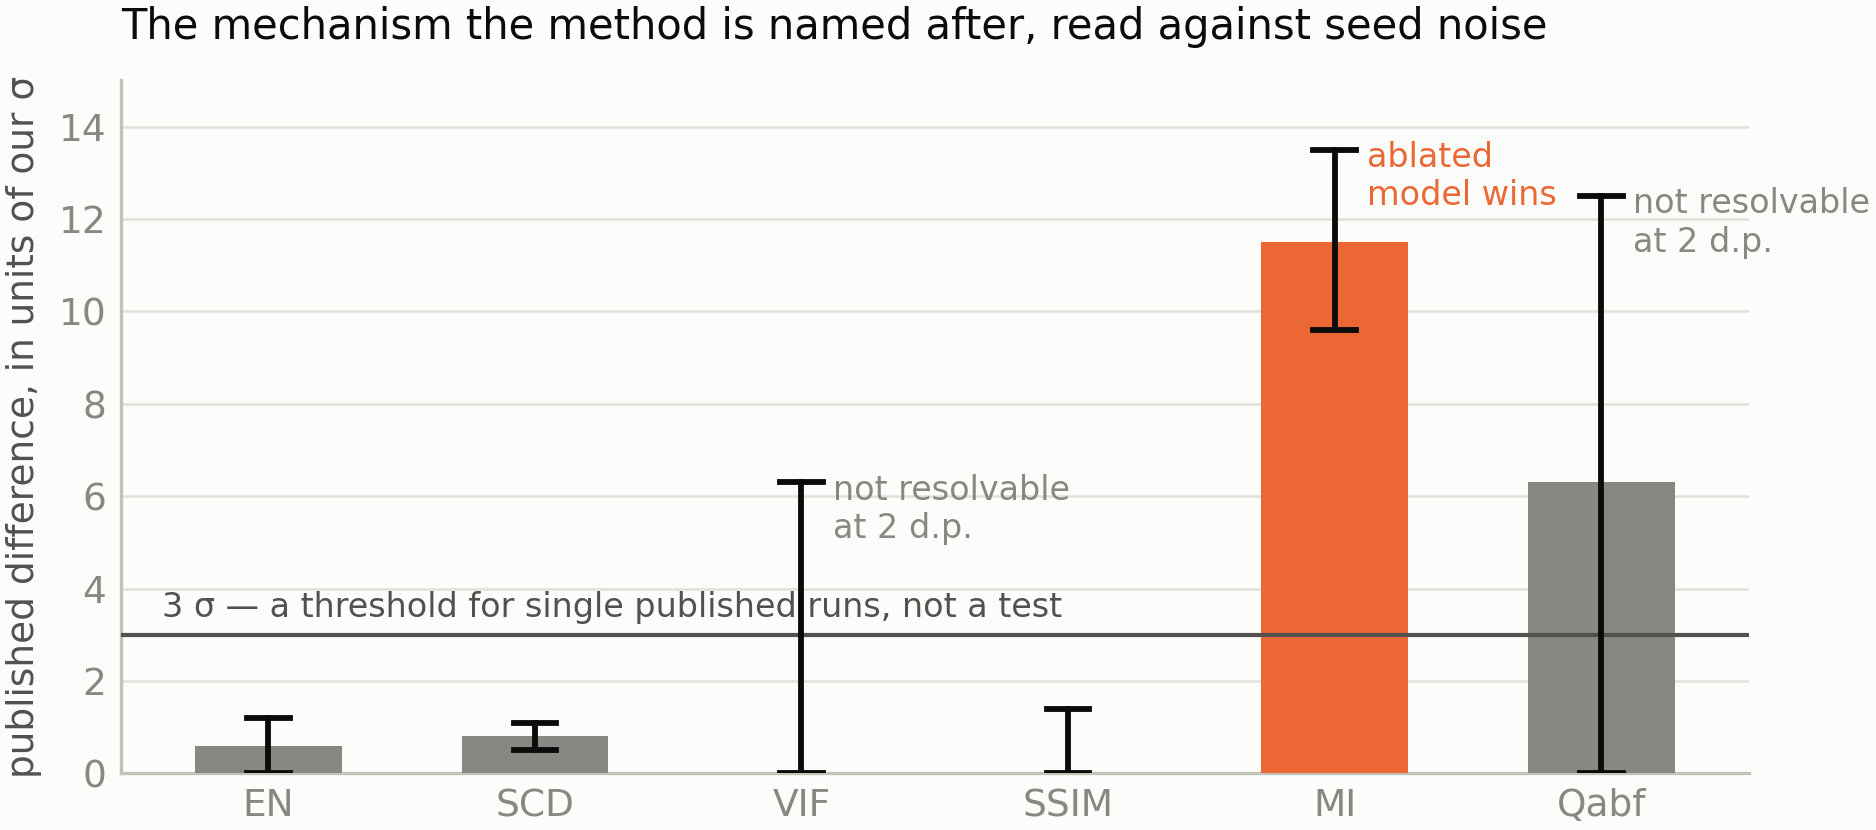
\includegraphics[width=0.92\linewidth]{fig_p4_row_i_vs_sigma}
\caption{The mechanism the method is named after, read against seed noise. \textbf{The values are the authors' own published numbers; $\sigma$ is measured here} (three retrained seeds of the paper's Eq.~(16) schedule) and was never reported by them. The line on each bar is the range consistent with two-decimal rounding: only MI exceeds the noise floor robustly, and it favours the model without the mechanism.}
\label{fig:p4_row_i_vs_sigma}
\end{figure}

$\sigma$ is the sample standard deviation of three retrained seeds of the configuration with the paper's Eq. (16) schedule; a comparison of the two spreads detected no difference between its spread and that of the released code, which is the basis for using it as the yardstick for variants that change loss and schedule. Row I of the published table \,---\, the ablation of the mechanism the method is named after \,---\, then reads as shown in Table \ref{tab:rowI}.

{\centering\footnotesize
\captionof{table}{Row I of CrossFuse's published ablation (the authors' values), read against $\sigma$ measured here.}\label{tab:rowI}
\begin{tabular}{llllll}
\toprule
Metric & Full & w/o Top-K & $\Delta$ in $\sigma$ & range at 2 d.p. ($\sigma$) & Verdict \\
\midrule
EN & 7.21 & 7.20 & 0.6 & 0--1.2 & noise \\
SCD & 1.70 & 1.67 & 0.8 & 0.5--1.1 & noise \\
SSIM & 0.99 & 0.99 & 0.0 & 0--1.4 & noise \\
VIF & 0.77 & 0.77 & 0.0 & 0--6.3 & not resolvable at 2 d.p. \\
Q$^{AB/F}$ & 0.54 & 0.55 & 6.3 & 0--12.5 & not resolvable at 2 d.p. \\
\textbf{MI} & 2.13 & \textbf{2.19} & \textbf{11.5} & \textbf{9.6--13.5} & \textbf{ablated model wins} \\
\bottomrule
\end{tabular}
\par}

The printed values carry two decimals, so each difference is uncertain by up to 0.01; the range column gives every value in $\sigma$ consistent with that rounding. Three differences (EN, SCD, SSIM) lie inside the noise floor at any such value, and two (VIF, Q$^{AB/F}$) cannot be resolved at the published precision. One, MI, exceeds the noise floor robustly, and it favours the model \emph{without} the mechanism, while the paper's stated justification rests on EN and SCD \,---\, two of the smallest differences in the row. \textbf{This result required no GPU time}: it combines the authors' published numbers with a precision they did not measure. Independent retraining also finds the model without Top-K ahead on MI on RoadScene, after Holm; on TNO, the test set of Row I, that verdict depends on which same-seed runs are used and is not claimed.

\subsection{The confound in the architectural ablations}

The table's two architecture rows substitute a Transformer block for a CNN block and vice versa. The substituted blocks are not the same size: the CNN is 15 \% of the Transformer it replaces, so one row removes 51 \% of the encoder and the other adds 51 \%. Each row therefore changes block \emph{type} and \emph{capacity} together.

Building the missing control is possible in one direction \,---\, widening the CNN until both encoders match within 0.08 \% \,---\, and it decomposes the reported effect into an architecture term and a capacity term. \textbf{The capacity term exceeds 3 $\sigma$ in 14 of 27 cells against 8 for the effect the row is used to demonstrate.} The confound is larger than the finding.

The control is also informative in its own right. At matched capacity the two blocks are not interchangeable: attention scores higher on VIF, Q$^{AB/F}$ and MI, and the deep CNN on contrast and sharpness (EN, SD, SF, AG). Equalising the parameter count does not equalise the function; it exposes a difference in inductive bias that the simultaneous size change had hidden. Two of the three measures on the attention side, MI and VIF, are the two that Section~7 shows reward a copy of the visible input on this architecture, so that side of the difference is not read as perceptual fidelity. The second architecture row cannot be capacity-matched \,---\, narrowing the attention block is bounded below by its projection dimensions \,---\, so its reading was pre-registered instead: it carries 51 \% more parameters and still loses on MI and VIF, so, if the added parameters do not themselves harm performance, the measured harm is a lower bound; Section~6 shows that this assumption can fail on another architecture, so the bound is conditional. It is also stated on MI and VIF, whose direction on this architecture Section~7 calls into question.

\subsection{Does the named mechanism buy stability?}

Removing Top-K is the table's own first row, and retrained at five seeds it does something the table cannot show: \textbf{seed-to-seed spread rises}, by a median factor of 2.17 over the released configuration, larger in 21 of 27 cells. The obvious reading is that the mechanism buys run-to-run stability, and we first wrote it down that way.

Code inspection led us to revise the claim because the implementation did not support its original interpretation. Top-K is not a module but a \textbf{data procedure}: it selects the auxiliary patches closest to the primary corpus in channel statistics, fits a per-channel gamma so their means match, and merges them in. The released training archive holds 918 primary and 800 auxiliary patches, so the published ablation, which sets k = 0, removes \textbf{47 \% of the training corpus} along with the mechanism. ``Top-K buys stability'' was never separable from ``more training data buys stability''.

A volume-controlled test separates them: the corpus is held at the same size in both arms, and the only difference is whether the auxiliary patches were drawn at random or selected and aligned by Top-K, at the k = 1000 CrossFuse publishes. It was run first, for cost, on the second architecture of this paper (LRRNet, 11,025 LLVIP pairs plus 1,000 MSRS patches). Selection was genuinely selective (mean channel distance 6.55 for the kept patches against 38.58 for the pool) and the fitted gamma came out at 1.011, so the mechanism ran as designed. \textbf{No effect was detected}, at three seeds per arm and again at \textbf{eight} in a registered extension (Run 27): no variance ratio of seven survives Holm, the point estimates lean the other way (Top-K more variable on all seven, median spread ratio 0.89, bootstrap interval 0.50--1.50), and no mean survives Holm (Top-K lower on EN, MI and VIF uncorrected). At eight seeds a variance ratio must exceed about 5 to reach significance (about 39 at three), and detecting a true ratio with 90 \% power needs about 14 (about 350 at three), so this is non-detection at a stated resolution; the point estimate does not favour the mechanism.

\textbf{And on CrossFuse itself.} The test was then repeated on CrossFuse with its own auxiliary source, as a registered run (Run 28). Both arms hold the released corpus's 1,718 patches: one is the authors' file, 918 RoadScene patches plus the 800 M3FD patches Top-K selected and gamma-aligned; the other keeps the same 918 RoadScene patches, byte for byte, and adds 800 M3FD patches drawn at random from the 5,729 in the pool, without alignment (mean channel distance to RoadScene 121.9, as for the whole pool, against 23.3 for the 800 closest). Five seeds per arm, the released training configuration. \textbf{No stability effect was detected here either}: no variance ratio of seven survives Holm on TNO (ratios 0.31--2.63; at five seeds a ratio must exceed about 9.6 to reach significance, and about 39 is needed for 90 \% power), and no mean survives Holm on any of the three test sets. Whether the 2.17$\times$ spread of the k = 0 ablation belongs to the mechanism or to the lost data \textbf{cannot be decided at this sample size}: the median spread ratio over the 27 cells is 1.00, but its bootstrap interval, 0.48--2.31, contains both no effect and the full k = 0 factor.

\textbf{Stated with its limit.} Three statements are strict: the spread increase measured in our retraining of the k = 0 row cannot be \emph{attributed} to the mechanism, because that design moves corpus size with it; a volume-controlled test detects no effect of the mechanism itself in either architecture family; and on CrossFuse, the attribution of the k = 0 instability remains open at five seeds per arm. An earlier attempt at k = 3610 from a pool of 5,415, which keeps two thirds of everything and is barely selective, appeared catastrophic; at the published k the catastrophe disappeared with the effect, so it measured our setting rather than the mechanism. Both are in the record.

\subsection{What holds in the paper's favour}

Reported with the same prominence as the criticism, because a protocol that only ever convicts is not a protocol. The checkpoint reproduces completely. A contamination suspicion was refuted by measurement rather than assumption: the train/test split was never released, but regenerating every candidate patch from the raw images recovered it exactly, and \textbf{no test-derived patch appears in training}.\footnote{181 training images and 40 test images, 918 candidate patches matched exactly, zero test-derived.} And substituting the blocks in either direction lowers the same two metrics, MI and VIF. Because Section~7 shows that these two reward a copy of the visible input on this architecture, this is consistent with the published assignment but does not establish it.

These findings do not indicate that the authors' architectural choices are flawed; rather, they show that single-run ablation deltas lack the measurement precision necessary to demonstrate those choices empirically.

\subsection{Findings the paper does not report}

Three, recorded because they bear on reproducibility rather than on quality. The released checkpoint holds 1,188,272 parameters against a stated 0.80 M; the released training script raises a \texttt{NameError} at import and could not have been executed as published; and the released training archive holds 800 patches from its auxiliary source while its auto-generated filename encodes 1,000, so the published artefact cannot have come from the published script at the stated setting. Section~8 returns to this class of defect, which recurs in case study II.

\subsection{A note on \texorpdfstring{$\sigma$}{sigma} for this study}

$\sigma$ here is the \textbf{sample standard deviation of three seeds}, not the eight-seed estimate of Section~5. With two degrees of freedom, its 95 \% confidence interval runs from about 0.5 to 6.3 times the estimate, so every figure in $\sigma$ units below inherits that width. It is the weaker of the two, and every figure quoted above should be read with that in mind: even the largest effect, 11.5 $\sigma$, would be about 1.8 $\sigma$ at the upper end of that interval, so no figure in $\sigma$ units here is decisive on its own, and the count of 14 of 27 cells inherits the same width. The MI result of Row I does not rest on this estimate alone: independent retraining, reported above, finds the model without Top-K ahead on MI on RoadScene after Holm. Differences in the 3--5 $\sigma$ band could be artefacts of the estimate. An earlier version of this section computed $\sigma$ as the \emph{population} standard deviation, which with three seeds is 0.82 of the sample value and inflated every figure above by a factor of 1.22; that is withdrawn claim \#13, and the values here are the corrected ones. The 3 $\sigma$ rule applied to single runs is a threshold, not a test: treated as a two-sided \emph{t}-test with the two degrees of freedom three seeds provide, the capacity term reaches the 5 \% level in 6 of 27 cells against 3 for the effect \,---\, the same ordering, on fewer cells. Where a conclusion depended on that band, a further seed was run, and twice it changed the conclusion.

\section{Case study II: an unrolled method, and a table re-measured entire}

The second testbed is LRRNet \citep{lrrnet}, chosen because it belongs to a different architectural family: it unrolls a low-rank-and-sparse decomposition rather than learning one, and carries 49,204 parameters against the first method's 1.19 M. A defect appearing in both is a property of how the field ablates, not of one design.

\textbf{Selection was by measurement, not by judgement.} Candidate cost was measured before commitment: CDDFuse \citep{cddfuse} needs 37.5 h per training run, so three seeds would take three to four weeks of the available quota (112.5 GPU-hours at 30 to 45 a week) \,---\, and its published \texttt{batch\_size} does not fit on the available hardware, nor on twice it. SeAFusion \citep{seafusion} was excluded from its configuration files alone, at no cost. LRRNet costs 1.10 h per run. That a published recipe is not executable on commonly available hardware is itself recorded, and it recurs below.

\subsection{Two findings before any training}

The block-count ablation compares 2, 4, 6 and 8 blocks at 29,744 / 49,204 / 68,664 / 88,124 parameters \,---\, a \textbf{2.96$\times$ capacity spread}. Block count and capacity move together, so no row difference is attributable to representational depth. This is the same defect as case study I's, in an unrelated architecture, and it was established without any training.

Second, and consequential for how the rest of the work was designed: \textbf{published IVIF metric values are not on a common scale.} LRRNet reports MI = 13.7 where our evaluator measures 2.50 on LRRNet itself; and CDDFuse's published SSIM = 1.03 is, in its own released evaluator, the \emph{sum} of two SSIM values on a scale to 2, which a reader of the table cannot know. In the evaluator used here, MI, VIF and SSIM are likewise summed over the two sources, and every comparison in this paper is made within that one evaluator. Comparing printed tables across papers without the evaluator is therefore unsafe, which forced every compared row here to be retrained rather than screened.

\subsection{\texorpdfstring{$\sigma$}{sigma}, and why recording a seed is not enough}

Five seeds of the published configuration give a genuine sample standard deviation. LRRNet is noisier than the first method on every metric \,---\, expected at four epochs against 160, and a property of the training budget rather than a defect.

A crash during the first attempt produced an unintended experiment: the same seed was trained twice, same code, same data. The two runs differ by up to \textbf{44 \% of $\sigma$} (median 16 \%), because cudnn remains free to select algorithms. \textbf{A paper reporting a single run together with its seed would still not be reproducible to the precision its own ablation table claims to resolve.}

\subsection{The table, re-measured entire}

\begin{figure}[t]
\centering
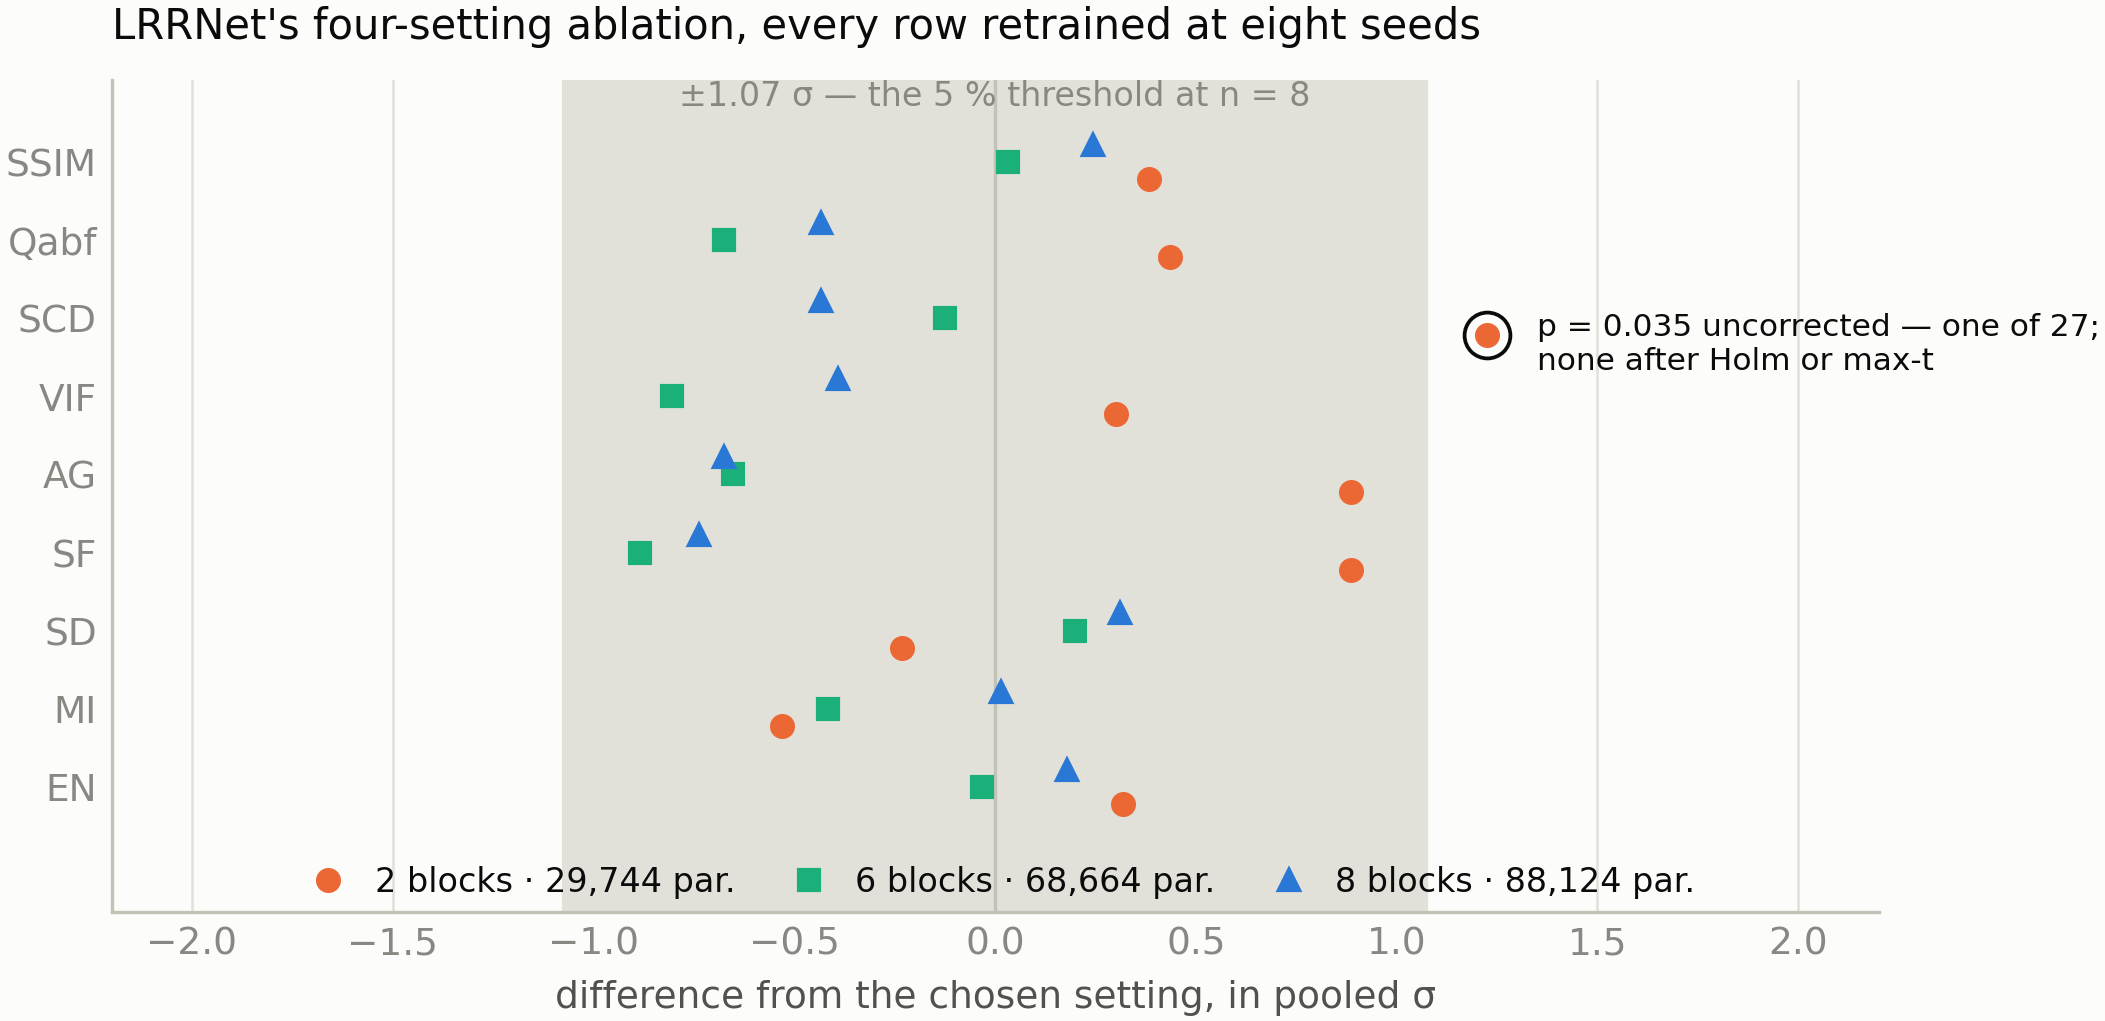
\includegraphics[width=0.92\linewidth]{fig_p3_table4_remeasured}
\caption{LRRNet's four-setting block-count ablation, every row retrained at eight seeds, one evaluator, the same 25 TNO pairs. One of 27 comparisons reaches the 5\,\% level uncorrected (SCD, 4 blocks against 2) and none survives a Holm correction; that cell did not replicate on twelve new seeds. The band is the significance threshold at $n=8$, not a fixed $\pm 3\sigma$ rule.}
\label{fig:p3_table4_remeasured}
\end{figure}

All four settings were retrained here \,---\, eight seeds each \,---\, scored by one evaluator on the same 25 TNO \citep{tno} pairs, against $\sigma$ measured on those same runs. No proxy is used anywhere; an earlier estimate that borrowed $\sigma$ across architectures is discussed below. The rows first stood at five and three seeds. All were taken to eight in a run whose reading \,---\, including the outcome that would withdraw this section's headline \,---\, was registered before it began.

\begin{quote}
\itshape \textbf{One of 27 comparisons reaches the 5 \% level} \,---\, SCD, 4 blocks against 2, $t = -2.45$ with a critical value of 2.26 \,---\, at the chance rate: re-assigning whole runs at random, a table with at least one such cell appears 56 \% of the time, and \textbf{none survives a Holm or max-\emph{t} correction.} Every difference lies inside 1.3 pooled $\sigma$, and the one significant cell favours the setting the paper's own numbers place lowest on most metrics.
\end{quote}

At three seeds per row the count was zero. It moved mainly because the correct threshold fell with the larger sample, not because the gap grew \,---\, but the gap does repeat in the five new seeds alone, so it is the one cell in the table that merited a follow-up registered in its own right, not a claim. \textbf{That follow-up was run, and the cell did not replicate.} Twelve new seeds per setting were trained, with the test fixed before any existed and the old seeds excluded from it, since they had produced the hypothesis: on the new seeds alone the gap is 0.54 pooled $\sigma$, $t = 1.33$, $p = 0.20$. The design had 82 \% power at the size first seen, but that size was selected for being the largest, so this shows the cell did not repeat at that size, not that the difference is zero.

Absence of significance is not equivalence, so the table is read that way too. At a margin of $\pm$1.75 pooled $\sigma$ \,---\, the resolution the run was registered to achieve, set before any of its seeds existed \,---\, \textbf{23 of the 27 differences are equivalent} by two one-sided tests. That test was chosen after the run: its registration fixed 1.75 $\sigma$ as the resolution the sample size buys, not as an equivalence margin, so this reading is a post hoc analysis at that margin; the follow-up below registered the same test in advance. Four were not: SCD, SF and AG against 2 blocks, and SF against 6 \,---\, \emph{inconclusive at eight seeds}. The same follow-up took settings 2, 4 and 6 to twenty seeds, and \textbf{at twenty seeds the four comparisons that were inconclusive at eight are all equivalent} within the registered $\pm$1.75 $\sigma$ margin, as are all 18 comparisons of settings 2 and 6 against the published four-block setting across the nine metrics. The twenty seeds include the eight that produced the inconclusive readings, so this is the second stage of a registered two-stage design, and no correction is made for the earlier look. None survives a Holm correction. Two of the four \,---\, SF and SCD against 2 blocks \,---\, are also nominally different at the 5 \% level: differences real enough to detect and smaller than the design resolves, reported as exactly that. Where this paper calls the settings indistinguishable, it means equivalent within $\pm$1.75 $\sigma$, and no more. The margin is the experiment's registered resolution, not a claim that differences below 1.75 $\sigma$ are practically negligible; an equivalence margin should ideally be set on what matters in the domain \citep{lakens}, and this field has not defined one.

The paper's justification for its chosen setting is that it ``obtains five best values''. Counted that way at eight seeds, 4 blocks leads 6 blocks on 7 of 9 metrics and 8 blocks on 5 of 9 \,---\, and trails 2 blocks on 7 of 9. \textbf{Not one of its leads is separable from run-to-run noise.} With nine correlated metrics and one run per setting a lead is nearly guaranteed to exist, and its existence says nothing about whether it is real. The chosen setting is then fixed for every other experiment in the paper.

\textbf{The published ranking of the four block-count settings is not reproduced either.} Two blocks is the setting the paper's own numbers place lowest on four of its six metrics (En, SD, MI and VIFm, in LRRNet's own labels), although highest on SSIMm. Retrained, it is nominally ahead of the chosen configuration on 7 of 9 metrics while using 60 \% of the parameters. We do not claim that 2 blocks is better: all but one of those differences is inside the noise band, the one that is not sits at the rate chance produces and did not replicate, and asserting a winner would repeat the same single-run inference in the opposite direction. The defensible statement is narrower and firmer \,---\, \textbf{retraining does not reproduce even the published ranking}, so the table's ordering carries no more information than its gaps do.

\textbf{In the paper's favour}, and stated as plainly: with four configurations indistinguishable on TNO, choosing the smallest is the correct engineering call. It is simply not the reason the paper gives, and not what its table demonstrates.

One further obstacle is recorded here and discussed in Section~8: \texttt{num\_block = 8}, one of the four settings the table compares, \textbf{exhausts a 16 GB card as released}, because the code pins itself to a single device and comments out its own multi-GPU line. Restoring that line is arithmetically neutral \,---\, the network contains no batch-dependent layer of any kind \,---\, and was chosen over a smaller batch, which would have made the row incomparable with the others. The deviations of Section~3 apply to every row above and are not repeated here.

\subsection{A second test set, the same checkpoints}

Every verdict above is measured on the 25 TNO pairs LRRNet's own paper uses. A null can be a property of a small test set rather than of the method, and the question costs no training: the 78 checkpoints behind this section and Section~6 were fused on RoadScene's 40 pairs and scored by the same evaluator, under a reading registered before any output existed. As a check that the pipeline is the one that produced the record, every checkpoint was also re-fused and re-scored on TNO in the same session: \textbf{all 702 TNO means reproduced the stored values to six decimals.}

\textbf{On RoadScene the table is no longer empty.} At twenty seeds, \textbf{four of 27 comparisons survive Holm correction}: 2 blocks is ahead of 4 on EN and SCD ($p = 0.0046$, $0.0047$), and 4 is ahead of 6 on VIF and SCD ($p = 0.0029$, $0.0059$); 8 against 4, at eight seeds, separates nothing. Holm is applied within each nine-metric comparison, the family registered for this run; under a single correction across all 27 comparisons none survives (smallest $p = 0.0029$ against a first threshold of $0.05/27 = 0.0019$), so these are differences detectable under the registered family, not a table-wide result. Every surviving difference is about one pooled $\sigma$, and all 18 twenty-seed comparisons remain equivalent within $\pm$1.75 $\sigma$ \,---\, twenty seeds resolve effects smaller than the design's equivalence margin, so these cells are both \emph{detectably different} and \emph{equivalent within the margin}, and are reported as exactly that.

Two readings follow, and we state both. \textbf{The ordering is the same on both test sets}: at twenty seeds, fewer blocks score higher, by about 0.7 to 1 $\sigma$. On TNO, 8 of the 18 comparisons of settings 2 and 6 against 4 reach $p < 0.05$ uncorrected, all in the direction \textbf{2 > 4 > 6}, and none survives Holm; a whole-run permutation (exploratory, chosen after the data were seen and not registered) gives a count that large in 18 of 100,000 reassignments. On RoadScene four survive Holm within each nine-metric comparison. What differs between the test sets is how far the same small effect clears correction, not its direction, and all 18 twenty-seed comparisons remain equivalent within $\pm$1.75 $\sigma$ on both. And the published justification fares no better: on neither set does the chosen setting lead the smaller one on any metric after correction, and on RoadScene the smallest setting is measurably ahead of it, at 60 \% of the parameters. The claim above that we do not call 2 blocks better stands for TNO after correction; on RoadScene it is better on two metrics, by about one $\sigma$. This withdraws a claim of our own (\#18 in Section~3).

The means behind both test sets, in the metrics' own units, for readers who need more than differences in $\sigma$ (mean $\pm$ sample SD over seeds) are given in Tables \ref{tab:means-tno} and \ref{tab:means-rs}.

{\centering\footnotesize
\captionof{table}{LRRNet's four block-count settings on TNO: mean $\pm$ sample standard deviation over seeds.}\label{tab:means-tno}
\begin{tabular}{lllll}
\toprule
TNO & 2 blocks (n = 20) & 4 blocks, published (n = 20) & 6 blocks (n = 20) & 8 blocks (n = 8) \\
\midrule
EN & 6.986 $\pm$ 0.023 & 6.981 $\pm$ 0.026 & 6.987 $\pm$ 0.029 & 6.984 $\pm$ 0.030 \\
MI & 2.449 $\pm$ 0.049 & 2.455 $\pm$ 0.095 & 2.453 $\pm$ 0.072 & 2.489 $\pm$ 0.039 \\
SD & 43.29 $\pm$ 0.82 & 43.70 $\pm$ 0.89 & 44.21 $\pm$ 1.14 & 43.98 $\pm$ 0.95 \\
SF & 10.91 $\pm$ 0.26 & 10.70 $\pm$ 0.28 & 10.54 $\pm$ 0.24 & 10.53 $\pm$ 0.22 \\
AG & 4.041 $\pm$ 0.119 & 3.966 $\pm$ 0.118 & 3.889 $\pm$ 0.091 & 3.870 $\pm$ 0.070 \\
VIF & 0.769 $\pm$ 0.022 & 0.752 $\pm$ 0.028 & 0.730 $\pm$ 0.022 & 0.747 $\pm$ 0.029 \\
SCD & 1.299 $\pm$ 0.026 & 1.265 $\pm$ 0.052 & 1.232 $\pm$ 0.046 & 1.237 $\pm$ 0.041 \\
Q$^{AB/F}$ & 0.436 $\pm$ 0.011 & 0.428 $\pm$ 0.012 & 0.420 $\pm$ 0.010 & 0.424 $\pm$ 0.017 \\
SSIM & 0.912 $\pm$ 0.010 & 0.908 $\pm$ 0.010 & 0.906 $\pm$ 0.011 & 0.909 $\pm$ 0.017 \\
\bottomrule
\end{tabular}
\par}

{\centering\footnotesize
\captionof{table}{LRRNet's four block-count settings on RoadScene: mean $\pm$ sample standard deviation over seeds.}\label{tab:means-rs}
\begin{tabular}{lllll}
\toprule
RoadScene & 2 blocks (n = 20) & 4 blocks, published (n = 20) & 6 blocks (n = 20) & 8 blocks (n = 8) \\
\midrule
EN & 7.229 $\pm$ 0.023 & 7.207 $\pm$ 0.023 & 7.194 $\pm$ 0.027 & 7.196 $\pm$ 0.033 \\
MI & 2.585 $\pm$ 0.040 & 2.563 $\pm$ 0.070 & 2.545 $\pm$ 0.054 & 2.572 $\pm$ 0.051 \\
SD & 49.06 $\pm$ 0.70 & 48.66 $\pm$ 0.85 & 48.33 $\pm$ 0.79 & 48.49 $\pm$ 0.84 \\
SF & 12.96 $\pm$ 0.26 & 12.74 $\pm$ 0.26 & 12.52 $\pm$ 0.27 & 12.52 $\pm$ 0.25 \\
AG & 4.618 $\pm$ 0.098 & 4.580 $\pm$ 0.096 & 4.509 $\pm$ 0.083 & 4.494 $\pm$ 0.104 \\
VIF & 0.677 $\pm$ 0.021 & 0.654 $\pm$ 0.030 & 0.628 $\pm$ 0.023 & 0.644 $\pm$ 0.034 \\
SCD & 1.533 $\pm$ 0.024 & 1.493 $\pm$ 0.053 & 1.447 $\pm$ 0.047 & 1.457 $\pm$ 0.043 \\
Q$^{AB/F}$ & 0.364 $\pm$ 0.006 & 0.359 $\pm$ 0.007 & 0.355 $\pm$ 0.006 & 0.357 $\pm$ 0.007 \\
SSIM & 0.792 $\pm$ 0.014 & 0.779 $\pm$ 0.019 & 0.771 $\pm$ 0.017 & 0.777 $\pm$ 0.025 \\
\bottomrule
\end{tabular}
\par}

\subsection{A calibration against our own earlier estimate}

Before these rows were trained, two of these comparisons were screened using $\sigma$ borrowed from case study I. That screen read them at 16.8 $\sigma$ and 3.90 $\sigma$ \,---\, ``clearly real''. Measured on LRRNet itself they are 0.74 $\sigma$ and 0.90 $\sigma$. \textbf{The borrowed estimate was wrong by more than twentyfold, in the direction that made the problem look smaller.} Borrowing $\sigma$ across corpora within one architecture proved defensible (1.19 $\sigma$ estimated against 0.51 $\sigma$ measured); borrowing it across architectures did not. This is reported against our own earlier number for the same reason the withdrawn claims of Section~3 are reported.

\section{Design for measurability}

Sections 4 and 5 criticise ablations whose confounds were controlled for badly or not at all. That invites an obvious reply: control them better. This section argues for something stronger \,---\, \textbf{design the architecture so the confound cannot be constructed} \,---\, and reports what happened when we did.

\subsection{Weight-tied unrolling}

LRRNet's core is described as an unrolled algorithm: one step of a solver, applied $\mathtt{num\_block}$ times. In the released code each application owns a separate set of learned weights, so it is not one step repeated but $\mathtt{num\_block}$ different steps. That is a departure from LISTA \citep{lista}, whose whole content is that the step is \emph{shared} across iterations \,---\, and it is precisely what makes the published block-count ablation unreadable, because depth and capacity then move together.

Tying the weights across iterations restores the algorithm and separates the two quantities (Table \ref{tab:params}).

{\centering\footnotesize
\captionof{table}{Parameter count of LRRNet with untied (released) and tied weights at each number of unrolled blocks.}\label{tab:params}
\begin{tabular}{llll}
\toprule
\texttt{num\_block} & untied & tied & reduction \\
\midrule
2 & 29,744 & 20,014 & 1.49$\times$ \\
\textbf{4 (published)} & \textbf{49,204} & \textbf{20,014} & \textbf{2.46$\times$} \\
6 & 68,664 & 20,014 & 3.43$\times$ \\
8 & 88,124 & 20,014 & 4.40$\times$ \\
\textbf{spread} & \textbf{2.96$\times$} & \textbf{1.00$\times$} &  \\
\bottomrule
\end{tabular}
\par}

Two properties follow. The model is \textbf{2.46$\times$ smaller} at the published setting; and the parameter count is \textbf{constant in depth}, so the parameter-count confound of Section~5 is not controlled for \,---\, it cannot be built.

Tying is off by default, and that default is verified rather than asserted: parameter names and shapes are compared tensor-by-tensor against unpatched upstream at four depths, so the eleven runs already reported remain reproducible from the same source file.

Trained on three seeds against the five-seed baseline, \textbf{0 of 9 metrics reach significance under the registered test}, and none differs by more than 1.6 pooled $\sigma$. Removing 29,190 parameters \,---\, 59 \% of the network \,---\, changes nothing that test can see, in a regime where, as Section~7 shows, the metrics have stopped registering further training by the second of four epochs. The result is scoped to that regime \,---\, and it survives twice the budget (below).

\begin{quote}
\itshape This comparison provides a proof of concept for confound-controlled depth ablation: tying unrolled weights removes the parameter-count confound by construction, yielding a 2.46$\times$ smaller model while demonstrating that, in this construction, depth can be varied while the parameter count remains fixed.
\end{quote}

\textbf{At five seeds against five} \,---\, a pre-registered extension that also removes the unequal-arm problem discussed below \,---\, \textbf{one metric of nine crosses uncorrected (SSIM, $p = 0.030$, in the tied model's favour) and none survives Holm.} By this paper's own definition of \emph{indistinguishable} (Section~5: equivalent within $\pm$1.75 pooled $\sigma$), equivalence is established for \textbf{two} metrics, EN and MI; the other seven are unresolved at five seeds \,---\, neither different nor shown equivalent. The accurate statement is therefore narrower than ``indistinguishable'': \textbf{2.46$\times$ fewer parameters, with no metric differing after correction.} The parameter count is the categorical half of the claim; the quality half is a null at the stated resolution (about 2 $\sigma$), not a demonstrated equivalence.

\textbf{Two things this does not license.} The tied model leads on 7 of 9 metrics \,---\, the same count Section~5 shows cannot support a conclusion \,---\, and none of those leads survives correction, so the verdict is \emph{no measured difference}, not \emph{better}. Relative spread also fell 1.98$\times$, which looks like a variance reduction; only 1 of 9 variance ratios clears $F(4,2)$, so it is recorded as a hypothesis and not a finding.

\textbf{The registered threshold was conservative, and one verdict depends on it.} The critical value 2.776 was fixed for this run as the value at df = 4; five seeds against three give df $\approx$ 5.6, where the exact value is 2.49. Recomputed at each comparison's exact degrees of freedom, one verdict of the 54 in Section~6 and Section~7 that used the fixed value changes: \textbf{SSIM, untied $\rightarrow$ tied at $d4$, $t = 2.70$, $p = 0.038$ \,---\, in the tied model's favour.} The registered reading is reported because it was registered; this one is reported beside it because a conservative threshold favours exactly the null this section states. It does not make the tied model \emph{better} \,---\, under Section~3 a single cell is not a result \,---\, but \emph{no difference} is the verdict of the registered test, not of every defensible one. At five seeds against five the same cell stands at $p = 0.030$ and still does not survive correction.

\subsection{The depth ablation the published table was presented as being}

\begin{figure}[t]
\centering
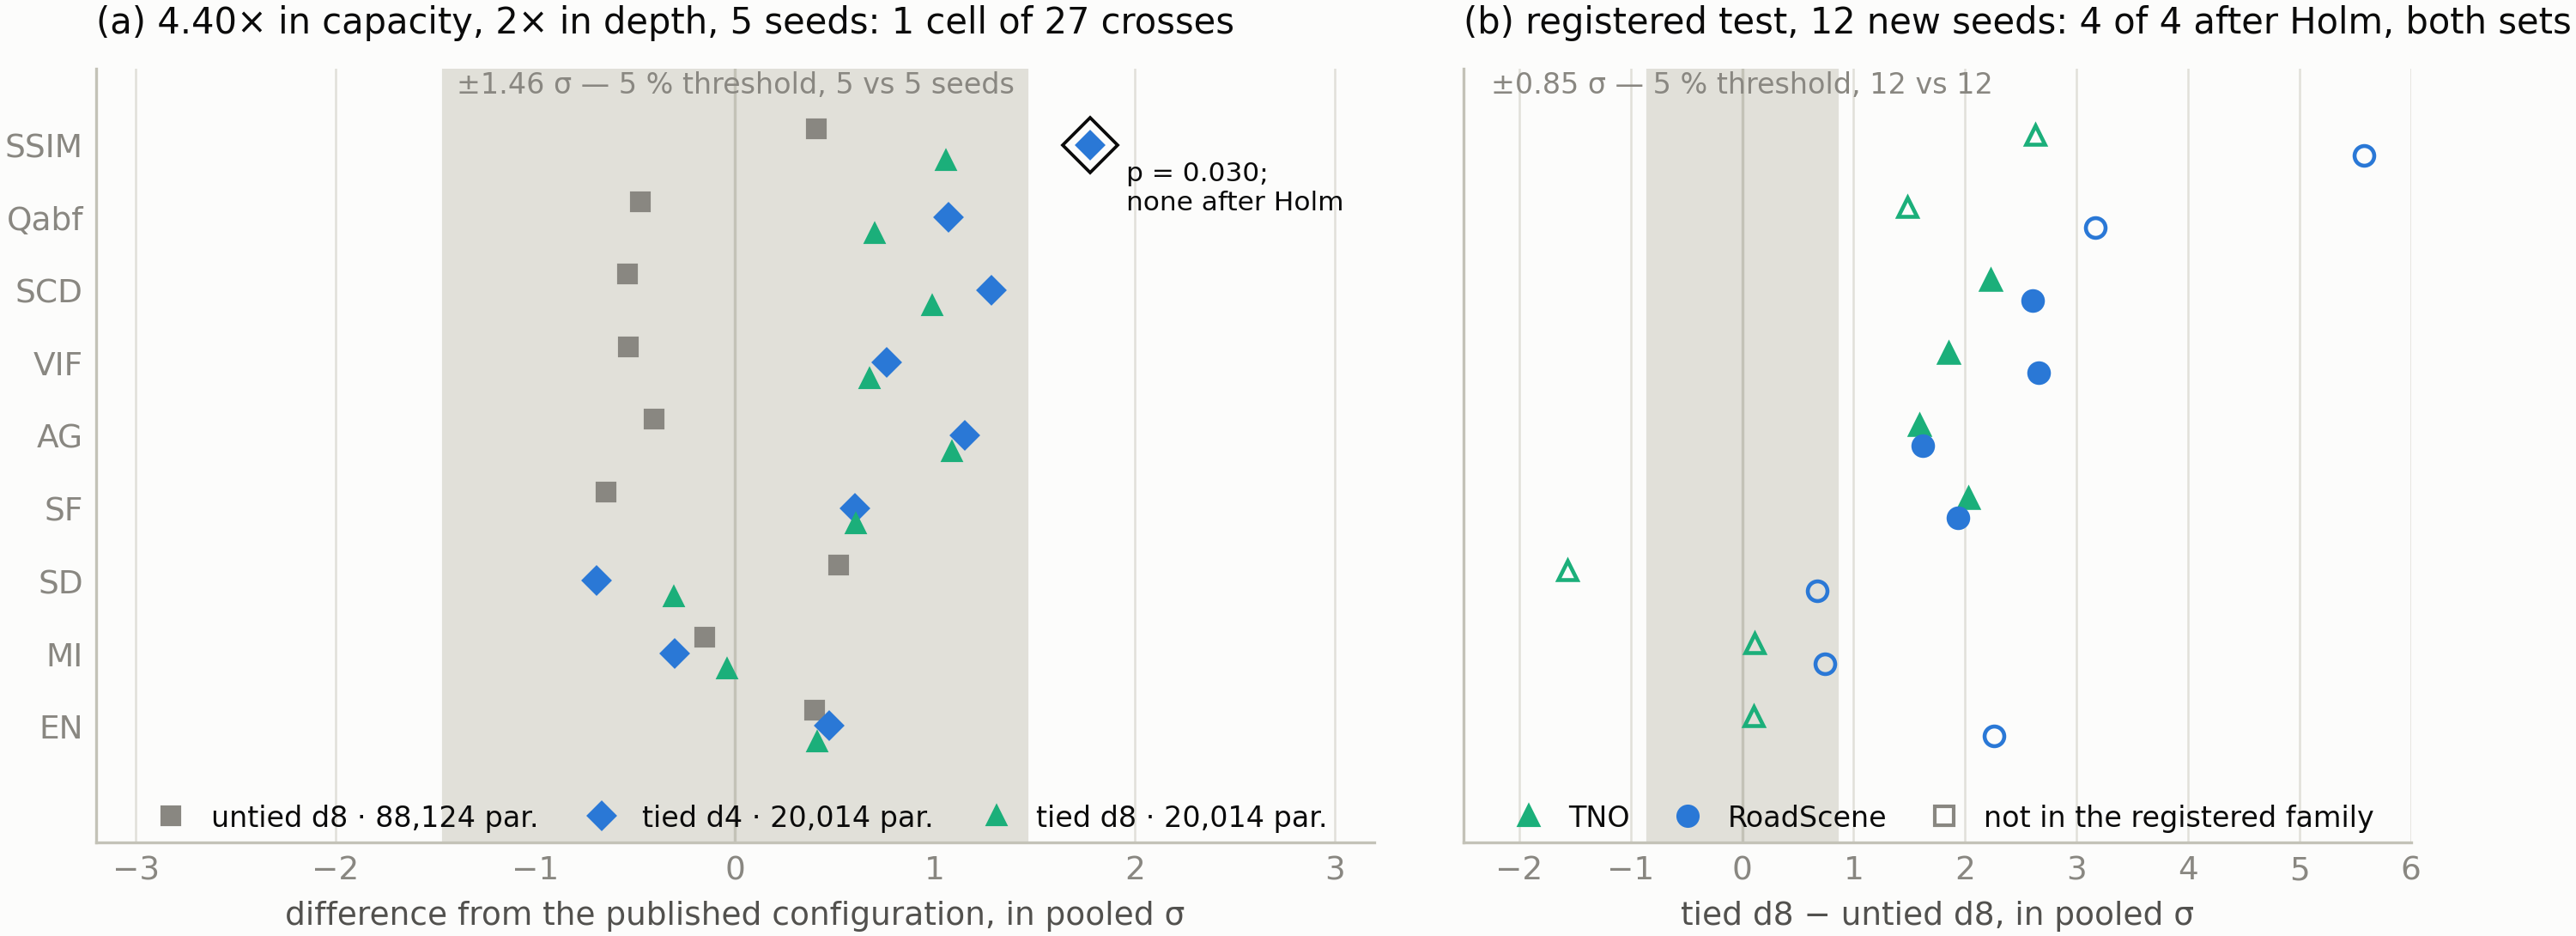
\includegraphics[width=0.92\linewidth]{fig_p5_capacity_by_construction}
\caption{Depth with the parameter count fixed. Weight tying makes the parameter count identical at depth 4 and depth 8, so depth varies with the parameter count held fixed by construction rather than controlled for after the fact. (a) Tied arms at five seeds, untied depth 8 at eight. Against the published configuration one cell of 27 crosses (SSIM, tied depth 4, $p = 0.030$); across all four contrasts of the $2\times2$, 5 of 36 cross uncorrected, four of them tied against untied at depth 8, all favouring the tied model and none surviving Holm; the band is the 5\,\% threshold for five seeds against five. (b) That contrast, registered and retested on twelve new seeds per arm and re-scored on RoadScene: the registered metrics (filled: SF, AG, VIF, SCD) all survive Holm on both test sets, favouring the 4.40$\times$ smaller tied network; open markers are descriptive, and SD on TNO is a cost. The band is the threshold for twelve against twelve.}
\label{fig:p5_capacity_by_construction}
\end{figure}

With the parameter count constant in depth by construction, eight iterations of the solver can be compared against four with nothing else different. Crossing depth with tying gives the $2\times2$ the published table needed and never had (Table \ref{tab:2x2}).

{\centering\footnotesize
\captionof{table}{The depth-by-tying 2$\times$2: metrics (of nine) that reach significance uncorrected in each contrast, at three and at five tied seeds.}\label{tab:2x2}
\begin{tabular}{>{\raggedright\arraybackslash}p{0.128\linewidth}>{\raggedright\arraybackslash}p{0.342\linewidth}>{\raggedright\arraybackslash}p{0.171\linewidth}>{\raggedright\arraybackslash}p{0.275\linewidth}}
\toprule
contrast & what it isolates & three tied seeds & five tied seeds \\
\midrule
tied $d4 \to d8$ & \textbf{depth, parameter count constant by construction} & \textbf{0 of 9} & \textbf{0 of 9} \,---\, 7 of 9 equivalent within $\pm$1.75 $\sigma$ \\
untied $d4 \to d8$ & depth \emph{as the published table measures it} (+38,920 par) & 0 of 9 & 0 of 9 \\
untied $\rightarrow$ tied at $d4$ & capacity, $-$29,190 par & 0 of 9 (1 at exact df: SSIM) & 1 of 9 (SSIM) \\
untied $\rightarrow$ tied at $d8$ & capacity, $-$68,110 par & 1 of 9 & \textbf{4 of 9} (SF, AG, VIF, SCD) \\
\bottomrule
\end{tabular}
\par}

\emph{Five tied seeds: Run 12 and Run 14, pre-registered; untied $d8$ at the eight seeds of Section~5. Every crossing cell favours the tied model and none survives Holm within its contrast.}

\textbf{The depth question has a clean answer, and it is a null.} Holding the parameter count fixed by construction, eight iterations of the solver against four move \textbf{0 of 9 metrics, and seven of the nine are shown equivalent} within $\pm$1.75 pooled $\sigma$ \,---\, the ablation LRRNet's Table IV was presented as being, and could not be, answered at five seeds.

\textbf{The capacity contrasts are where the table leans.} With three tied seeds the $2\times2$ counted 1 of 36 cells at the registered threshold (2 at exact df), inside the 1.8 expected by chance. With five it counts \textbf{5 of 36} (8 if untied $d4$ is also taken to its eight seeds), and four of them sit in one contrast: \textbf{at depth 8 the tied network is nominally ahead of the untied one on SF, AG, VIF and SCD} ($p$ = 0.021, 0.007, 0.008, 0.017). None survives Holm, so under Section~3 this is not a result \,---\, and because it favours this paper's own model, the rule is applied without exception. But ``consistent with chance'' no longer describes the count. What the table shows is that removing 68,110 parameters at depth 8 costs nothing measurable and may help; claiming it would need its own registered test.

\textbf{That test was run, and the lead replicated.} The four metrics that raised the question were fixed as the confirmatory family, the seeds that raised it were excluded, and twelve new seeds per arm were trained. At depth 8 the tied network (20,014 parameters) is ahead of the untied one (88,124) on \textbf{all four after Holm correction} \,---\, SF +2.03 $\sigma$ (+0.50, +4.8 \%), AG +1.59 $\sigma$ (+0.18, +4.8 \%), VIF +1.85 $\sigma$ (+0.060, +8.2 \%), SCD +2.23 $\sigma$ (+0.096, +7.9 \%), every $p \le 0.0011$ \,---\, and on \textbf{RoadScene}, scored from the same checkpoints under a reading registered before any of them had been fused there, on all four again, by more (+1.62 to +2.66 $\sigma$). Descriptively it is also ahead on Q$^{AB/F}$ and SSIM, and \textbf{behind on SD} ($-$1.57 $\sigma$ on TNO, $-$1.58 in SD's own units, $-$3.6 \%): less global contrast, reported as a cost. The mechanism the numbers point to is the one the $2\times2$ already hinted at \,---\, depth \emph{hurts} the untied network, and tying prevents it: descriptively, untied depth 8 scores below untied depth 4 on these metrics (a gap LRRNet's Table IV did not resolve), while tied depth 8 shows no detected difference from tied depth 4 (Run 14).

\textbf{Against the published configuration itself}, the tied depth-8 network \,---\, 2.46$\times$ smaller than it \,---\, was first registered for comparison on RoadScene only, because its TNO comparison had already been seen. On RoadScene it is better on \textbf{six of the seven} metrics that pass LRRNet's positive control after Holm (EN, MI, VIF, SCD, Q$^{AB/F}$, SSIM; +1.1 to +3.2 $\sigma$) and worse on none. On a third test set, MSRS (361 pairs), under a reading registered before any checkpoint was fused there, it is better on \textbf{four} (EN, VIF, Q$^{AB/F}$, SSIM; +1.5 to +1.9 $\sigma$), SD and SCD are shown equivalent, and none is against it; it also stays ahead of the untied depth-8 network there on SF, AG and VIF. On TNO, read before these registrations and so exploratory, it was a trade-off: better on VIF and SSIM, worse on SD. A general test followed: \textbf{twelve further new seeds} of the tied network against eight seeds of the published configuration that had entered none of these comparisons, TNO and RoadScene read together under one registered rule, which named in advance a trade-off as a possible outcome. That is the outcome it returned. On RoadScene the tied network is better on EN, VIF, Q$^{AB/F}$ and SSIM (+1.6 to +2.6 $\sigma$) with none against; on TNO it is better on VIF, Q$^{AB/F}$ and SSIM (+1.4 to +1.9 $\sigma$) and \textbf{worse on SD} ($-$1.83 $\sigma$). It keeps the infrared target that Section~7 shows MI and VIF will pay a network to discard (TNO pair 02: 1.05$\times$ the published contrast). The defensible sentence is the scoped one, now at independent seeds: \textbf{weight tying makes depth usable \,---\, a network 2.46$\times$ smaller than the published one is better than it on RoadScene and MSRS, and on TNO trades global contrast (SD) for VIF, Q$^{AB/F}$ and SSIM.} A general improvement is not claimed.

To quantify effect sizes beyond threshold testing, Table \ref{tab:ci} provides exploratory 95 \% confidence intervals (Welch intervals, expressed in units of pooled $\sigma$ across both arms) for the registered comparisons. Every effect that survived Holm has an interval excluding zero. The lower bounds lie between 0.4 and 1.8 $\sigma$, so the effects are real and could be as small as about half a $\sigma$.

{\centering\footnotesize
\captionof{table}{Exploratory 95 \% confidence intervals (Welch) for the registered comparisons, in units of pooled $\sigma$.}\label{tab:ci}
\begin{tabular}{>{\raggedright\arraybackslash}p{0.224\linewidth}l>{\raggedright\arraybackslash}p{0.638\linewidth}}
\toprule
Comparison (seeds) & Set & Effect in $\sigma$, 95 \% CI \\
\midrule
tied d8 $-$ untied d8 (12 vs 12) & TNO & SF +2.0 [1.2, 2.9]; AG +1.6 [0.7, 2.4]; VIF +1.8 [1.0, 2.7]; SCD +2.2 [1.4, 3.1] \\
tied d8 $-$ untied d8 (12 vs 12) & RoadScene & SF +1.9 [1.1, 2.8]; AG +1.6 [0.7, 2.5]; VIF +2.7 [1.8, 3.5]; SCD +2.6 [1.7, 3.5] \\
tied d8 $-$ published d4 (12 vs 8) & TNO & VIF +1.8 [0.6, 2.9]; Q$^{AB/F}$ +1.4 [0.4, 2.4]; SSIM +1.9 [0.8, 2.9]; SD $-$1.8 [$-$2.9, $-$0.8] \\
tied d8 $-$ published d4 (12 vs 8) & RoadScene & EN +2.2 [1.3, 3.1]; VIF +1.6 [0.6, 2.7]; Q$^{AB/F}$ +2.0 [0.8, 3.1]; SSIM +2.6 [1.4, 3.8] \\
\bottomrule
\end{tabular}
\par}

For the published-configuration comparison, the remaining metrics' intervals include zero (TNO: EN, MI, SCD; RoadScene: MI, SD, SCD).

\subsection{Does the smaller network have headroom the published one lacks?}

Every comparison so far is at the published budget of four epochs, and that budget saturates the metrics (Section~7). A design claim owes the question whether the tied network, 2.46$\times$ smaller, gains more from training than the network it replaces. Both were trained at \textbf{twice the budget}, five seeds each, with three families of nine comparisons and their readings registered before any kernel existed. The training loss is still falling at eight epochs on both networks (seed 44's epoch mean, tied: 57,151 at epoch 4, 56,181 at epoch 8), so the manipulation took (Table \ref{tab:budget}).

{\centering\footnotesize
\captionof{table}{Twice the training budget (eight epochs against four): metrics that separate the arms after Holm correction and uncorrected.}\label{tab:budget}
\begin{tabular}{lll}
\toprule
family & after Holm & uncorrected \\
\midrule
tied@8 vs tied@4 & \textbf{VIF lower at 8} ($-$3.43 $\sigma$, $p = 0.002$) & VIF, Q$^{AB/F}$, both lower \\
untied@8 vs untied@4 & 0 of 9 & 0 of 9 \\
tied@8 vs untied@8 & 0 of 9 & AG, SCD, SSIM \,---\, all favouring tied \\
\bottomrule
\end{tabular}
\par}

\textbf{Doubling the budget improves no metric on either network, and it lowers VIF on both} \,---\, measurably on the tied network, whose seed spread in VIF is a sixth of the untied one's; the untied network's fall is larger in absolute terms and inside its noise. By the reading registered in advance this is recorded as a measured cost of longer training for the tied network. It is not a cost of tying: at eight epochs the tied network is behind the untied one on no metric. \textbf{The headroom is not in the budget.} With depth (0 of 9, seven equivalent) and capacity (no metric after correction), that is three independent directions in which nothing buys quality \,---\, so the contribution of this section is what it claimed at the outset and no more: the same algorithm at 2.46$\times$ fewer parameters, with the confound unbuildable.

\subsection{An asymmetric refinement, and why it failed}

Section~4 established, at matched capacity, that attention and CNN blocks are not interchangeable. LRRNet computes a low-rank half and a sparse half and then processes both with an \emph{identical} layer, so the measured assignment ought to apply.

The parameter budget makes the test clean. Tying freed 29,190 parameters; spending exactly those on an attention refiner for the low-rank half and a CNN refiner for the sparse half returns the model to 49,204 \,---\, identical to the published network. Over $d,e \in [4,96]$ that constraint has \textbf{exactly one solution} among 8,649 candidate pairs, so the widths are determined by the budget rather than chosen. Both refiners are residual with zero-initialised output projections and are constructed last, so at a given seed the refined model begins from the \emph{same} weights as the unrefined one \,---\, visible in the logs as an initial training loss of 296,583 against 296,780. The comparison is therefore \textbf{paired}, which removes the seed noise the two runs share.

\textbf{0 of 9, paired.} And the prediction fails \emph{directionally}: MI was predicted to rise and fell in every one of three seeds.

Two explanations remain and this experiment cannot separate them. The assignment may not transfer to a split the architecture never enforces \,---\, $L$ and $S$ are two channel slices of one tensor, with no rank constraint anywhere in the forward pass \,---\, or the attention bottleneck may simply be too narrow at the width the budget forces. \textbf{Widening it would tune against the budget that makes the comparison capacity-matched}, so it can only ever be a separate, declared experiment, and is listed as such.

A cost worth stating: the refined model runs \textbf{17 \% slower at identical parameter count}. Matching parameters is not matching compute, and a claim of equal size that omits runtime hides a real difference.

\section{The positive control}

Most results reported so far are null results. Each is ambiguous between two readings \,---\, \emph{the intervention did nothing}, and \emph{the metrics cannot see} \,---\, and nothing above distinguishes them. A reader is entitled to suspect the second, and until this section nothing rules it out.

We therefore adopt the parameter-randomisation test of \citet{adebayo}, developed for saliency methods: score a trained network against the same architecture with random weights. A measure that does not separate them gives no evidence that it measures the network. Why a randomly initialised network is a fair sensitivity control for a fusion metric: it changes nothing but the learned parameters (architecture, input pipeline, test images and evaluator are held fixed), and it is the largest degradation of a network that still produces an image. A metric meant to rank fusion networks by quality should rank a network that learned nothing below one that did, in the right direction and with the number of runs an ablation table uses; if it does not, its ranking of trained variants of that architecture carries no demonstrated meaning. Passing is necessary, not sufficient: it shows the metric responds to gross failure, not that it resolves the small effects an ablation looks for, which is what the milder arms probe. Three degradations were run at five seeds each, in decreasing severity: an \textbf{untrained} network (weights verified tensor-by-tensor against a freshly seeded model, zero gradient steps), \textbf{half the training budget}, and \textbf{a quarter of the unrolled depth} at identical parameter count.

The three degradations were run on LRRNet, the cheaper testbed at 1.10 h per run. \textbf{The untrained and half-budget arms were then repeated on the second architecture}, because a claim about what a metric can measure should not rest on one network \,---\, and because our own reading of each was written down before the run. Table \ref{tab:control} summarises the outcome.

{\centering\footnotesize
\captionof{table}{The positive control: metrics (of nine) that separate each degraded arm from the trained network, on both architectures.}\label{tab:control}
\begin{tabular}{>{\raggedright\arraybackslash}p{0.470\linewidth}>{\raggedright\arraybackslash}p{0.107\linewidth}>{\raggedright\arraybackslash}p{0.357\linewidth}}
\toprule
what was broken & detected (LRRNet) & detected (CrossFuse) \\
\midrule
untrained \,---\, random weights, no training & \textbf{7 of 9} & \textbf{9 of 9} \\
half the training budget (2 vs 4 epochs on LRRNet, 150 vs 299 on CrossFuse) & 0 of 9 & \textbf{2 of 9} after Holm (3 uncorrected), five seeds per arm \\
depth 1 instead of 4, same parameters & 0 of 9 & \,---\, \\
\bottomrule
\end{tabular}
\par}

On CrossFuse, the trained and half-budget arms use the step-matched configuration without Top-K (918 RoadScene patches; 299 and 150 epochs; Section~4), the configuration of the k = 0 arm, which reuses two of these runs as seeds. The inversion reported below does not depend on that choice: the released checkpoint scores MI 2.16 and VIF 0.764 on TNO, also below the untrained network (3.47 and 0.945).

\textbf{Both repeated arms disagreed with the first architecture}, and neither disagreement is the one we expected. That is the section's main result.

\subsection{Two metrics fail on one architecture and lead on the other}

\begin{figure}[t]
\centering
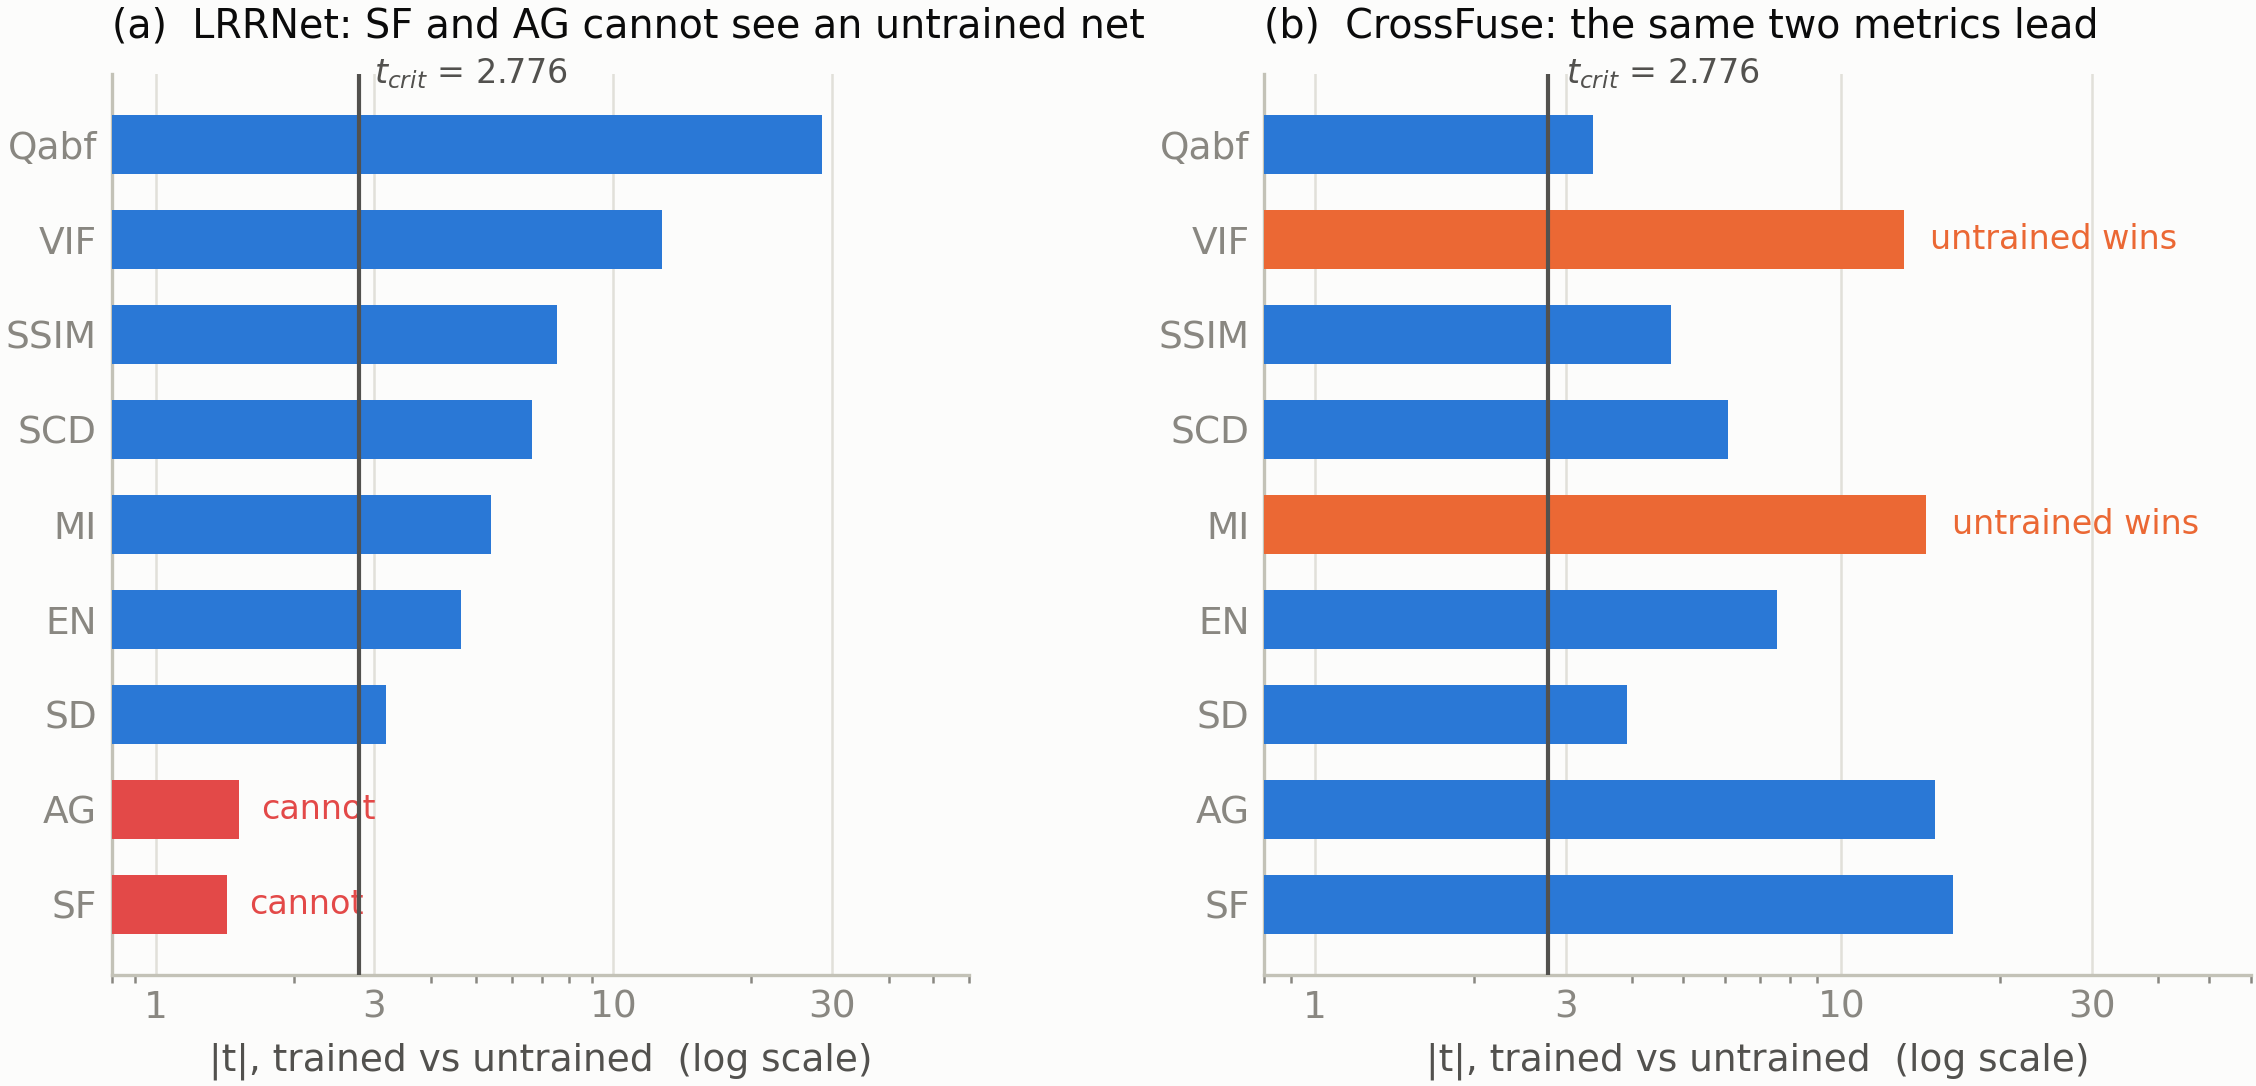
\includegraphics[width=0.92\linewidth]{fig_p1_positive_control}
\caption{The positive control of \citet{adebayo} on both architectures, five seeds per arm, metrics in the same order in each panel. \textbf{SF and AG cannot separate an untrained LRRNet from a trained one, and are the strongest detectors of all on CrossFuse}; MI and VIF pass on LRRNet but rank the untrained network \emph{above} the trained one on CrossFuse (orange). Whether a metric responds is a property of the metric and the network together, so a control cannot be assumed to carry over from another paper.}
\label{fig:p1_positive_control}
\end{figure}

Per-metric results are in Figure \ref{fig:p1_positive_control}; the full tables are released with the code and data (see Code and data availability).

\textbf{SF and AG did not separate random weights from a fully trained LRRNet} at five seeds per arm ($|t| = 1.43$ and $1.52$ against a critical 2.776). The means are far apart; the untrained arm's variance absorbs them, and it \emph{grows} with sampling ($\pm$2.94 on SF at n=5 against $\pm$2.36 at n=3). One untrained seed scored AG = 4.24 against the trained model's 4.06. A third, \textbf{SD, requires five seeds}. A metric that cannot separate an untrained model from a trained one cannot be treated as a validated ablation instrument on that architecture; one needing five training runs to notice cannot be used in a table reporting a single run. Non-separation at five seeds is not equivalence: the means are far apart, and what fails is the metric's ability to resolve them at the sample sizes ablation tables use. A registered follow-up at \textbf{twenty seeds per arm} gave the same reading: after Holm neither separates (uncorrected p = 0.029 and 0.026), and at the measured spreads about \textbf{forty runs per arm} would be needed for 90 \% power, against two to seven for the other seven metrics.

On \textbf{CrossFuse}, \textbf{nine of nine detect \,---\, and SF and AG are the strongest of them}, at $t = 16.34$ and $15.04$.

The two architectures fail differently because their untrained outputs differ. LRRNet's is a high-frequency mess whose gradient energy lands near a trained network's while varying wildly across seeds \,---\, exactly what defeats a gradient statistic. CrossFuse's is a near-copy of the visible image (measured below), whose gradient energy sits well under a trained network's in every seed \,---\, which those same statistics separate decisively and with almost no spread.

\begin{quote}
\itshape \textbf{The failure is a property of the metric--architecture pair, not of the metric.} We had written the opposite reading down as plausible \,---\, SF and AG are gradient statistics, so the mechanism looked general \,---\, and this run refutes it. The consequence is not weaker than the claim it replaces: \textbf{a metric's ability to respond did not transfer between the two architectures measured here, so it cannot be assumed to carry over from another paper's experiment. Every architecture--metric pair an ablation claim rests on should be validated by its own responsiveness control.} Two architectures show that transfer can fail; they do not show how often it does.
\end{quote}

\subsection{Two metrics rank the untrained network \emph{above} the trained one}

\begin{figure}[t]
\centering
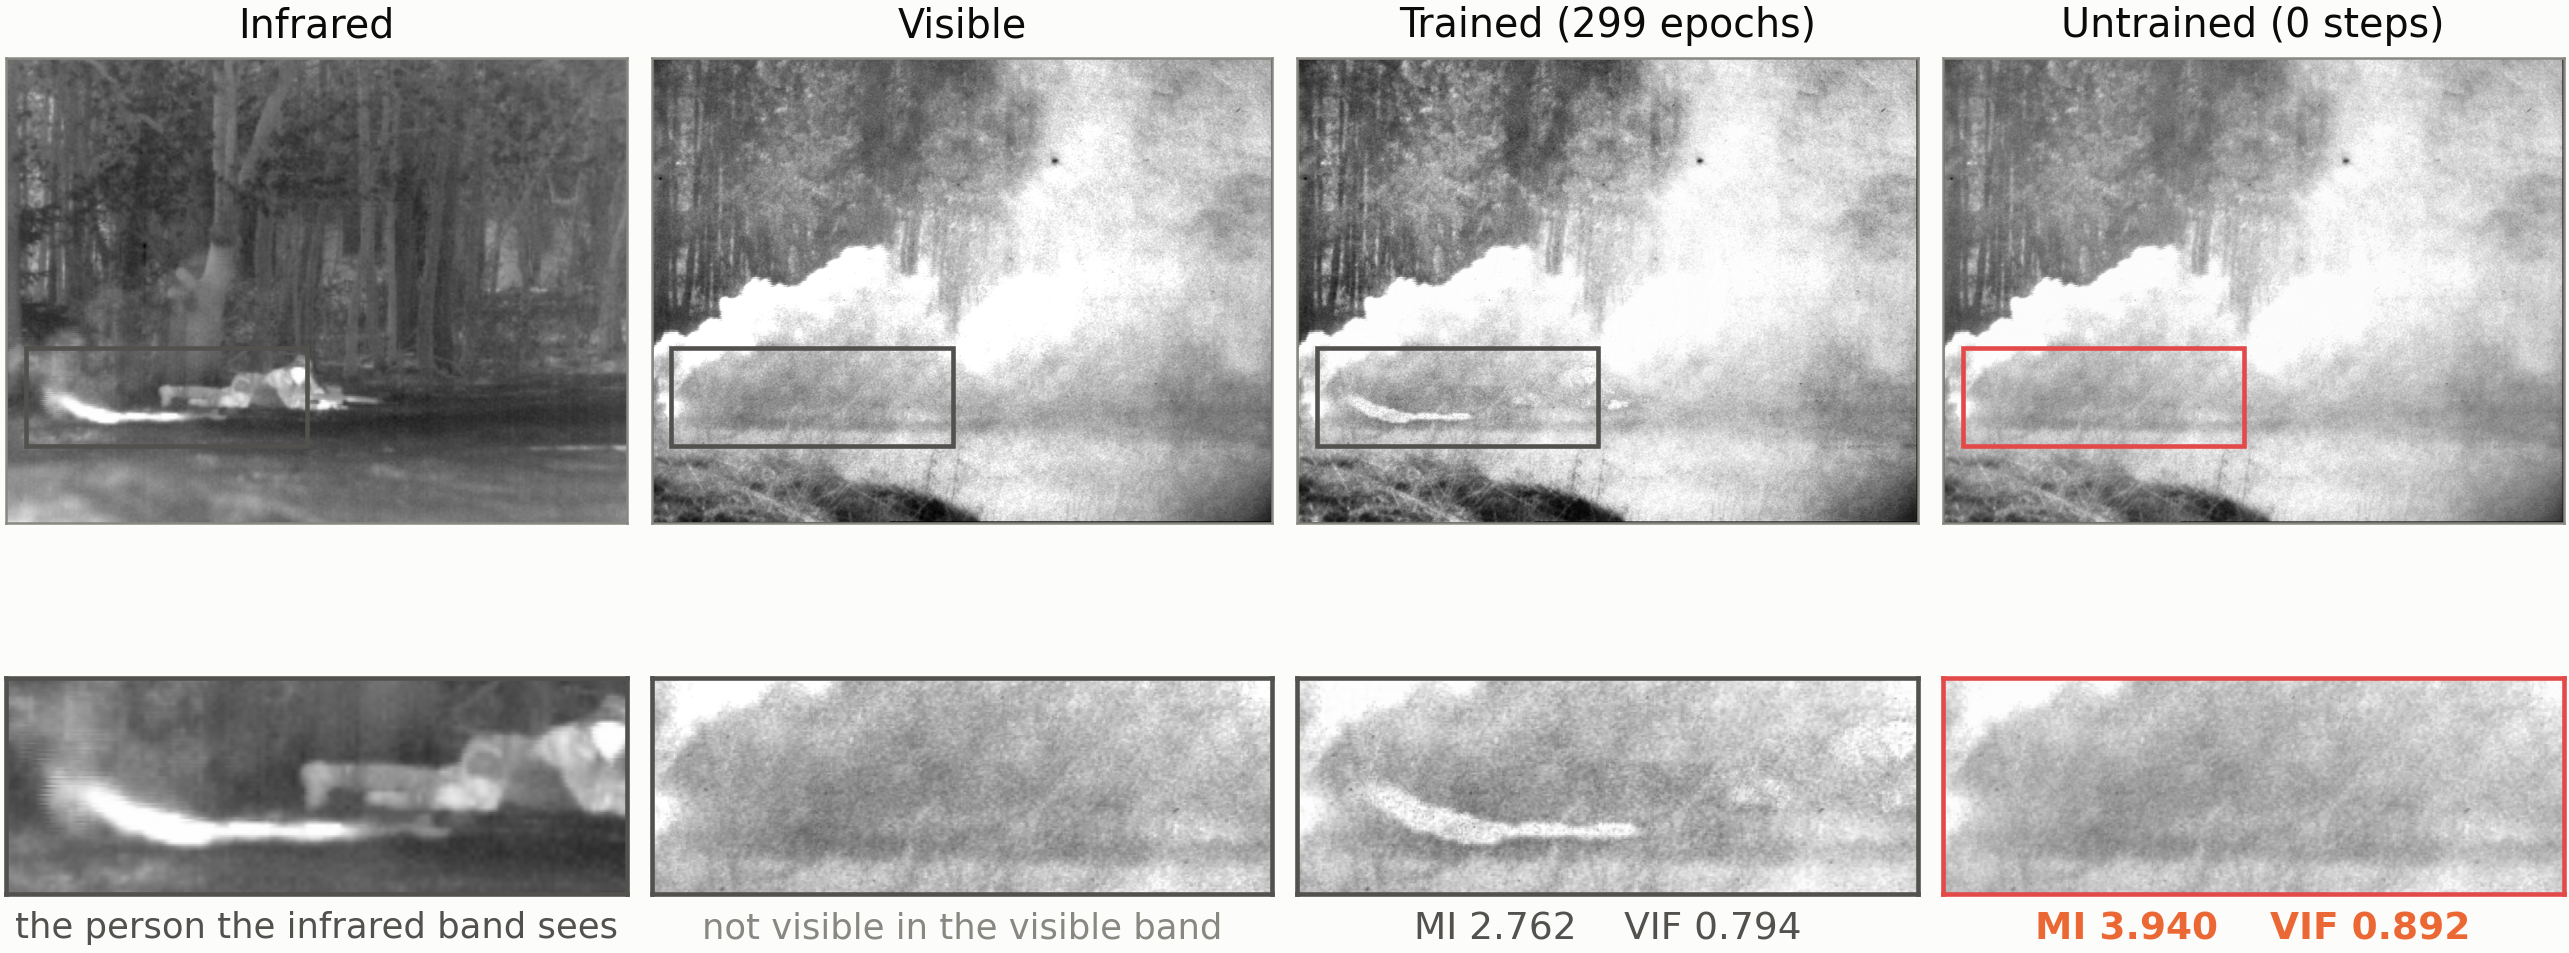
\includegraphics[width=0.92\linewidth]{fig_p6_untrained_qualitative}
\caption{What MI and VIF prefer. TNO pair 02: the infrared band holds a person lying in the grass and the visible band does not show them. The trained network carries them through; the untrained network returns the visible band -- r = 0.999 on this pair -- and loses them entirely. (The trained output is close to the visible band here too, r = 0.985, because it carries most of this scene; what separates them is the person.) \textbf{Both metrics score the image without the person higher} -- MI 3.940 against 2.762, VIF 0.892 against 0.794. Across all 25 pairs the visible band copied unchanged scores higher still (\S7): these measures reward reproducing a source, and fusion earns its name by departing from both. Across all 25 pairs and five untrained seeds the output matches the visible band at r = 0.996--0.998, against about 0.79 for a trained network, returned by the decoder's residual connection. Fused with the same checkpoints as the table above.}
\label{fig:p6_untrained_qualitative}
\end{figure}

On CrossFuse, MI and VIF do not merely fail to prefer the trained model \,---\, they prefer the untrained one, decisively and in every seed. An untrained network scores \textbf{MI 3.47 against 2.30} and \textbf{VIF 0.945 against 0.784}.

We had an explanation \,---\, the untrained network's output is close to a passthrough of the sources, and both measures reward agreement with them \,---\, and it was tested before being printed, against zero-network baselines, with the reading written into the script beside the code. \textbf{In its averaging form it fails.} The plain average of the two sources scores \textbf{MI 1.60 and VIF 0.57}, far \emph{below} the trained network (withdrawn claim \#12, Section~3). What the two measures reward is not blending but \emph{copying}: the visible image returned unchanged scores \textbf{MI 5.16 and VIF 1.04}, and the infrared image 4.96 and 1.03 \,---\, above both trained networks and above the untrained one. That VIF can favour a model that returns a source has been remarked in passing, in Section 4.2 of \citep{hybrid-fusion}, from one method whose output was essentially its infrared input; what is added here is the controlled measurement, on MI as well, and the mechanism below. The inversion is therefore a property of the measures rather than of this network, and a stronger one than the network result shows: \textbf{a ``fusion'' that fuses nothing outscores both trained networks on MI and VIF.} \textbf{Where an untrained CrossFuse falls was then measured, with the reading committed before the run.} Its decoder adds the visible input back before the output \,---\, \texttt{sigmoid(conv(features) + visible)} \,---\, so with random weights the learned branch contributes little and the output should be close to a copy of the visible image. Fusing the 25 TNO pairs with all five untrained checkpoints, whose fused images reproduce the originally scored ones exactly, confirms it: each output correlates with the visible image at \textbf{r = 0.996--0.998}, against 0.64--0.69 for the average of the sources and 0.64--0.67 for their pixel-wise maximum. A trained CrossFuse moves away from the visible image (r $\approx$ 0.79). \textbf{The inversion is a residual connection returning its input, scored by two measures that reward exactly that} \,---\, a property of a decoder that adds one modality back, not of fusion networks as such.

\textbf{CrossFuse inherits that decoder from CDDFuse} \citep{cddfuse}, so the account was tested there too, with the reading committed before the run. CDDFuse's released checkpoint, fused and scored by its own code, reproduces its published TNO row on all eight of its metrics. Five untrained CDDFuse networks return the visible image at r = 0.997 and outscore it on MI (3.47 against 2.19) and VIF (0.945 against 0.768; one-sample $t = 16.0$ and $15.2$, df = 4), while five of its other six metrics rank the released model higher. The inversion holds against the released models of both methods. It is not an independent replication on the untrained side: CrossFuse carries CDDFuse's encoder and decoder, built from the same seeds in the same order, and the two untrained arms agree on every shared metric to within 0.002. What is shown is one decoder lineage, outranking the trained models of both published methods that use it; whether an unrelated design with an input skip inverts the same way is not tested.

\textbf{The account also makes a prediction that could fail: a network with no path from its input to its output cannot return a copy, and so should not invert.} We tested it on a released method from outside that lineage, again with the reading committed before any output existed. SeAFusion \citep{seafusion} (two encoders, concatenation, four decoder convolutions and a $\tanh$ output \,---\, no input skip) was run with its released checkpoint and its own test-time processing against five untrained networks, scored by the same evaluator on the same 25 TNO pairs. The untrained outputs copy nothing (mean r to the visible image $-$0.12, against 0.997 for the two skip architectures), and \textbf{MI and VIF rank them far \emph{below} the released model} ($t = -55.4$ and $-229.8$, df = 4); eight of the nine metrics separate the arms. A second candidate, DenseFuse \citep{densefuse}, could not be read: its released pipeline clamps and casts to eight bits without normalising, so an untrained DenseFuse \,---\, whose outputs stay below 2 of 255 \,---\, renders as the same black image for every seed, and a kill criterion registered in advance stops the reading there. Across the architectures measured, \textbf{the inversion appears in the two with the skip and in neither without it} (LRRNet, SeAFusion). That supports the mechanism; it does not show the skip is the only route to an inversion.

Figure \ref{fig:p6_untrained_qualitative} is what that looks like. On one TNO pair the infrared band holds a person lying in the grass, invisible in the visible band; the trained network carries them through and the untrained network loses them. \textbf{Both metrics score the image without the person higher.} The failure is not subtle once seen, and it is not a corner case: it is the ordinary behaviour of a measure that rewards agreement with the sources in a task whose whole purpose is to discard some of that agreement.

\textbf{A metric that ranks an untrained network above a trained one is worse than one that cannot tell them apart}, and it is worse in a way a single-architecture study could not have found: on LRRNet both metrics pass. Any ablation table whose conclusion rests on MI or VIF for a network with this decoder is resting on a measure that rewards doing less.

\subsection{The other two arms: no detected difference}

For LRRNet, halving the training budget and reducing unrolled depth to one quarter both yielded no metric separations (0 of 9). Inspection of the training trajectories indicates that this reflects metric saturation after the second epoch rather than metric insensitivity: at seed 43, the logged loss at two epochs was comparable to that at four (58,219 vs. 58,549), and at seed 42 depth 1 matched depth 4 within 0.5 \% (57,909 vs. 57,634). The loss does not stop falling \,---\, at twice the budget it is still declining slowly, 1.7 \% from epoch 4 to 8 at one seed (Section~6) \,---\, but no metric follows it: no metric separates the arms (0 of 9), consistent with the metrics no longer registering further training by the second epoch. This is non-detection at the tested sample sizes, not demonstrated equivalence across all metrics; that distinction had to be checked rather than assumed, and checking it reversed the first reading we wrote down.

\begin{quote}
\itshape With the parameter count identical at depths 1, 4 and 8 by construction, \textbf{no metric separates the three depths after correction, and their training losses are comparable at the tested settings}. The evaluation therefore \textbf{detects no advantage of eight iterations over one} at the tested sample sizes, while eight cost 88 \% more compute per epoch. That is a result about the idea the architecture is named after, not about a setting inside it.
\end{quote}

\subsection{Sample-size sensitivity and claim refinement}

This table first stood at three seeds per arm and read ``three metrics cannot detect an untrained network''. It had already been written up when we noticed that our own standard condemned it: a headline claim resting on three seeds, in a paper about claims resting on too few seeds. Two seeds were added to both arms, with the reading of every outcome \,---\, including \emph{the finding narrows} \,---\, fixed in the notebook before the run.

It narrowed. SD reversed, and the wording was withdrawn everywhere it appeared.

\textbf{It then narrowed a second time.} The finding above \,---\, two metrics failing \,---\, was written up as a claim about \emph{the metrics}. The limitation that it rested on one architecture was stated, and the experiment that would settle it was named with its cost. Running it cost the claim its generality: on CrossFuse the same two metrics are the strongest detectors of all. The wording was narrowed again, and the recommendation that replaced it is stronger than the one it lost.

\subsection{What the control settles}

\begin{figure}[t]
\centering
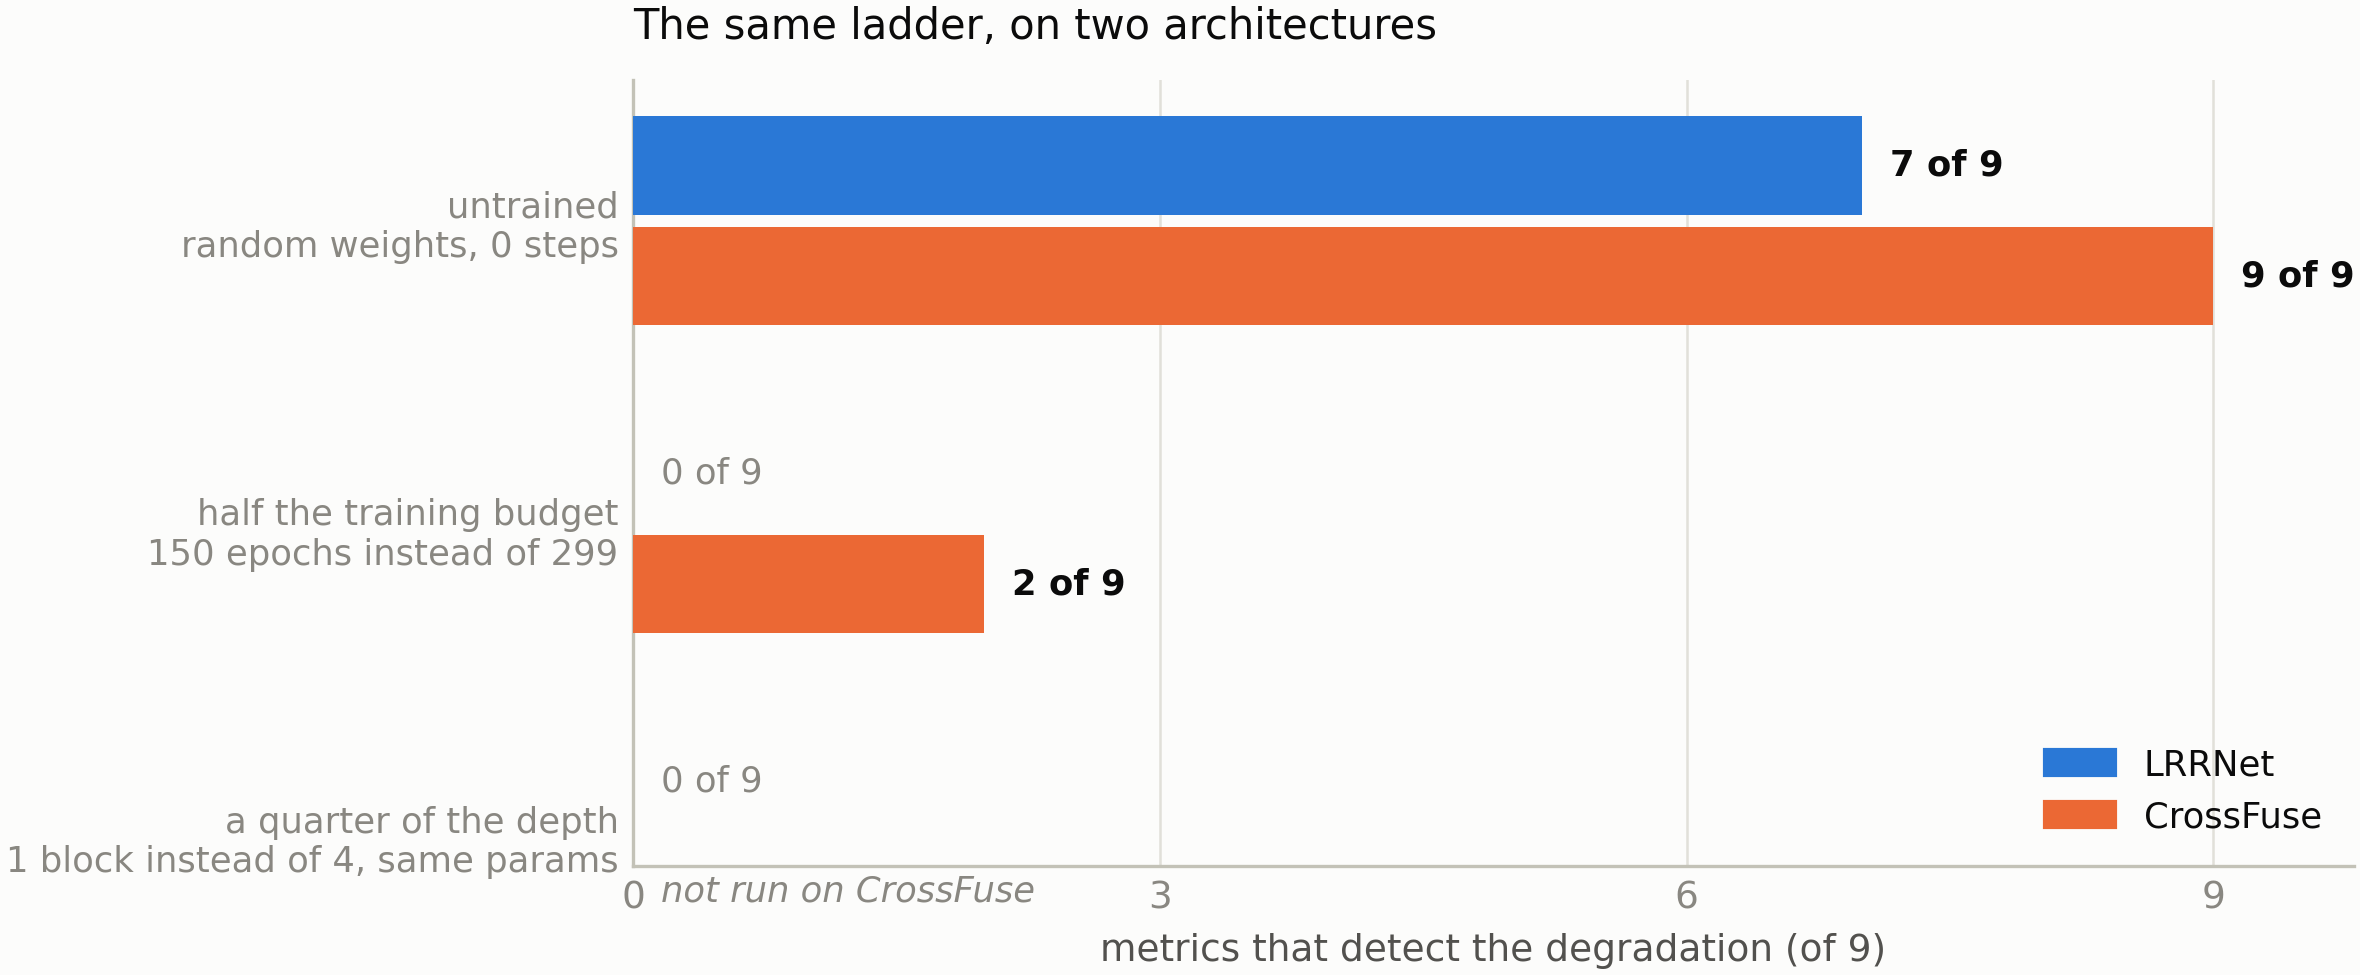
\includegraphics[width=0.92\linewidth]{fig_p2_sensitivity_ladder}
\caption{The same three-arm ladder on both architectures. On LRRNet the sensitivity floor lies between total failure to train and half the training budget, and the ablations re-measured here live inside that gap; its two lower arms show no detected difference, with comparable training losses. On CrossFuse the halved budget IS resolved -- but only by MI and VIF, the same two that rank an untrained network above a trained one. The floor belongs to the metric-architecture pair, not to the metrics.}
\label{fig:p2_sensitivity_ladder}
\end{figure}

Three things, of increasing consequence. \textbf{The nulls of Section~5 and Section~6 are not caused by total unresponsiveness} \,---\, 7 of 9 metrics respond to gross failure on the architecture those nulls were measured on. That does not show sensitivity at the effect sizes those ablations probe (the half-budget and depth-1 arms resolve none of the nine), so the nulls are read only at their stated resolution, through equivalence tests. \textbf{The resolution is enormous on LRRNet}: there, between total failure to train and half the training budget, these measures resolve nothing at all. On CrossFuse two of the nine do resolve it \,---\, and \emph{which} two is the finding. \textbf{MI and VIF are the only metrics that separate 150 epochs from 299 after correction, and they are the same two that rank an untrained CrossFuse above a trained one.} At five seeds per arm (pre-registered; Welch at exact df, Holm across nine) both survive ($p = 0.0006$ and $0.005$); a third, Q$^{AB/F}$, crosses only uncorrected ($p = 0.026$) and is named rather than counted. MI and VIF are also the only two whose ordering across the three arms is non-monotone with both legs significant; Q$^{AB/F}$'s untrained mean sits on its half-budget mean, and four other metrics print an out-of-order mean whose half-versus-full leg is inside the noise band, so none of them is read. So the measures that behave sensibly detect \emph{gross failure to train} and, at most weakly, how much training happened, while \textbf{the only two with corrected resolution in that range are the two that prefer no training at all.} Either way, on these two architectures, a table that swaps one block type for another cannot resolve what it claims to measure.

\textbf{And a control cannot be borrowed} \,---\, whether a measure responds is a fact about the measure \emph{and} the network it scores, so it must be established where it is used. Two arms have now been repeated on a second architecture and both changed their answer. That is the cheapest experiment in this paper, and none of the tables we examined runs it.

\section{Discussion}

\subsection{What the measurements say together}

Across two architecture families, four published ablation comparisons and three of our own modifications, the pattern is consistent: \textbf{almost nothing we changed moved a metric beyond the noise of retraining.} Capacity varied 4.40$\times$, depth 2$\times$, one headline mechanism was removed, another added, and the count of significant comparisons stayed near what chance alone produces, with one exception: the tied network at depth 8, whose lead over the untied one was confirmed by a registered test on new seeds (Section~6).

The positive control tells us how to read that. The metrics do respond to a network that was never trained \,---\, decisively, for seven of nine on LRRNet and for all nine on CrossFuse. On LRRNet they do not respond to halving the training budget, and the training losses show why: \textbf{the models reach comparable training losses}, because the metrics stop registering further training by the second epoch \,---\, at twice the budget the loss still falls slowly and no metric rises (Section~6) \,---\, and one iteration of the unrolled solver does the work of four. So the nulls are not total blindness, but on that architecture the resolution of the instrument sits somewhere between \emph{total failure to train} and \emph{half the training budget} \,---\, an enormous gap, and the ablations re-measured here live inside it.

On CrossFuse the same arm resolves the halved budget, but only through \textbf{MI and VIF}, the two metrics that also rank an untrained network above a trained one. The gap is therefore not a fixed property of the nine measures. It is narrower on one architecture than the other, and where it narrows, it does so through the two measures whose direction cannot be trusted. Neither reading rescues an ablation that swaps one block type for another: on one architecture nothing in that range is resolved, and on the other it is resolved only by measures that prefer no training at all.

\subsection{Three defects, and only one is about statistics}

These are properties of how the field reports ablations, not lapses particular to the two methods studied: every method reviewed reports its table the same way, and the two were chosen for their architectures, not for their tables.

\textbf{Variance is unreported.} This is the cheap defect: three or five training runs and a standard deviation would fix it, and the practice is standard elsewhere \citep{henderson,bouthillier,colas}.

\textbf{Confounds are structural, not accidental.} Both papers' architecture ablations change block type and parameter count together, in one case by $\pm$51 \%, in the other across a 2.96$\times$ range. This cannot be repaired by more seeds. It is repaired either by building the matched control \,---\, which we did, and which showed the confound larger than the effect it was used to demonstrate \,---\, or by designing so that the confound cannot exist, which Section~6 shows is available for unrolled architectures, at no parameter cost.

\textbf{No control establishes that the instrument responds.} This is the defect with no cheap fix, because on each architecture we tested, two of the nine standard metrics fail it \,---\, \textbf{and not the same two, nor in the same way:} on one, two metrics do not respond; on the other, two different metrics respond in the wrong direction. SF and AG did not separate random weights from a fully trained LRRNet after correction, even at twenty seeds (each nominally significant, p $\approx$ 0.03); on CrossFuse they are the strongest detectors of all, while MI and VIF there rank the untrained network \emph{above} the trained one.

That is the finding with the widest reach in this paper. \textbf{Whether a measure responds is a property of the measure and the network together}, so it cannot be established once and cited thereafter. A table whose conclusion rests on a metric is worth no more than that metric's demonstrated ability to respond \emph{on that architecture}, and the only way to know is to run the control there. It costs one evaluation of an untrained model, and none of the tables we examined runs it.

\subsection{A recurring failure that is not about measurement at all}

Twice in this work a \emph{published configuration could not be executed as published}: one method's stated batch size does not fit the hardware it claims, and one of the four settings its own ablation table compares exhausts a 16 GB card because the released code pins itself to a single device and comments out its own multi-GPU line. A third released training script raises an error at import and therefore cannot ever have produced the checkpoint shipped beside it.

\textbf{A table can contain a row a reader cannot reproduce at all} \,---\, a failure prior to any question of significance, and one that no amount of statistical care in the reader would surface.

\subsection{What this does not license}

Our analysis does not demonstrate that the published methods are technically ineffective. In both cases, the underlying architectural directions remain viable: CrossFuse's block allocation is consistent with the matched-capacity control but not established by it, because that control reads it on MI and VIF, whose direction Section~7 questions on that architecture, and LRRNet's configuration selection represents a sensible engineering choice given that larger variants do not yield measurable gains. The limitation lies strictly in the evidentiary value of single-run tables, which cannot establish these conclusions with the precision they assume.

Nor does it license the reverse error. Our own re-measurement, at eight seeds per row, shows a setting the published table places worst leading on 7 of 9 metrics \,---\, six inside the noise and one, SCD, at the rate chance produces, which did not replicate on twelve new seeds \,---\, and therefore not a finding. Asserting a winner from it would repeat the same single-run inference in the opposite direction.

\subsection{What we would ask of a table}

Table \ref{tab:steps} lists six steps, none of them expensive, each guarding against a failure measured in this paper.

{\centering\footnotesize
\captionof{table}{Six steps for an ablation table, the failure each guards against, and its cost.}\label{tab:steps}
\begin{tabular}{>{\raggedright\arraybackslash}p{0.107\linewidth}>{\raggedright\arraybackslash}p{0.600\linewidth}>{\raggedright\arraybackslash}p{0.144\linewidth}>{\raggedright\arraybackslash}p{0.066\linewidth}}
\toprule
Step & What to do & Guards against & Cost \\
\midrule
1. Measure the noise floor & Retrain the reference configuration at three seeds or more (five preferred); report mean and standard deviation per metric, with the seeds and the code version; if exact reruns matter, enable deterministic algorithms (about 20 \% slower on LRRNet) & a difference smaller than retraining noise (Section~3, Section~5) & 2 to 4 extra runs \\
2. Decide by a test & Test each difference at the design's own degrees of freedom and correct across the metrics (Holm); never decide by a fixed band in $\sigma$ & a lucky cell among nine correlated metrics (Section~5) & none \\
3. Read nulls as equivalence only when shown & Use two one-sided tests at a stated margin; otherwise report ``inconclusive'' and state what the sample size resolves & no evidence read as evidence of no effect (Section~3, Section~5) & none \\
4. Hold size fixed & When a component's type changes, match the parameter count, or state the confound's direction & capacity mistaken for architecture (Section~4, Section~6) & one control run \\
5. Run a positive control & Score an untrained copy of the same architecture with the same metrics; flag any metric that does not separate it from the trained model as unvalidated for that architecture, and do not use it alone to support an ablation claim there & a blind metric, or one that prefers a copy of an input (Section~7) & one evaluation, no training \\
6. Fix the reading first & Write down what each possible outcome will mean before the run & interpretation chosen after the numbers (Section~3) & none \\
\bottomrule
\end{tabular}
\par}

The fifth step is the one this work would insist on most: run on a second architecture to confirm a result, the control reversed it.

\section{Limitations and conclusion}

\subsection{Limitations}

\textbf{Sample sizes are small.} The complete ablation of Section~5 stands at eight seeds per row (twenty for three of its four settings) and resolves 1.75 $\sigma$; outside the complete ablation and its registered follow-ups, sample sizes vary by experiment; the initial studies commonly used five seeds for the reference configuration and three per ablated row, and each result states its own sample size. A variance estimate at n = 3 is weak \,---\, F(2,2) needs a variance ratio near 39 (two-sided 5 \%) to reach significance, and a mean difference below 3.5 $\sigma$ cannot be resolved at 90 \% power (the table in Section~3) \,---\, and every claim about spread is qualified accordingly. This bound is not incidental: it is the same constraint the papers under study operate under, and it is why conclusions here rest on several metrics agreeing rather than on any one.

\textbf{One method's corpus could not be rebuilt.} Its loader takes an unspecified 20,000-file prefix of a folder whose construction is never described, and no file list was released, so LLVIP substitutes for KAIST. Our numbers describe that architecture and procedure on that data. They are never compared against the authors' printed values \,---\, which the metric-scale result in Section~5 shows would be unsound in any case.

\textbf{One reading uses the authors' printed values.} The Top-K row of CrossFuse's table (Section~4) is read as published, against $\sigma$ measured here; independent retraining also finds the model without Top-K ahead on MI, on RoadScene. No other comparison uses a printed value. The $\sigma$ it is read against was measured on our retrains, which never reach the released VIF, so the authors' own run-to-run spread may differ.

\textbf{Inference is over training randomness, on fixed test sets.} Every test treats a run's mean over a fixed set of test pairs as the unit, so $\sigma$ describes retraining, not the sampling of test images. The two can disagree: the complete ablation is null on TNO's 25 pairs after correction, though the same ordering appears there uncorrected, while on RoadScene (40 pairs) four of the 27 cells survive correction within their nine-metric families. A nested resampling of runs and images would bound both, and is not done here.

\textbf{Determinism was deliberately not enforced}, so the measured $\sigma$ captures run-to-run variability under that execution setup and does not isolate the contributions of seed-driven and hardware-driven variability. That is a choice: $\sigma$ must describe what a reader re-running the released code meets, and forcing determinism would understate it \,---\, making more published differences look real, which would weaken the argument this paper makes.

\textbf{Two explanations remain unseparated.} The asymmetric refinement of Section~6 produced a null that is consistent either with the block assignment failing to transfer, or with an attention bottleneck too narrow at the width the parameter budget forces. Widening it would tune against the budget that makes the comparison size-matched, so the question is left open and named rather than resolved by an edit.

\textbf{One control arm still runs on one architecture.} The untrained and half-budget arms were both repeated on the second testbed; \emph{a quarter of the depth} was measured on LRRNet only. The half-budget repeat is what removed the larger version of this limitation, and it did so by contradicting us: the resolution floor is not a property of the metrics, it is a property of the metric--architecture pair, and it moved when the architecture did. The depth arm is the same shape as the experiments already run and is left named rather than assumed away.

\textbf{The metric--architecture interaction is demonstrated, not explained.} We show that SF and AG fail on one network and lead on another, and that MI and VIF invert on the second. The mechanism first offered for the inversion \,---\, that an untrained CrossFuse approximates a passthrough \,---\, was tested against zero-network baselines and failed in its averaging form; a copy of the visible input, delivered by the decoder's residual connection, was then measured directly (r = 0.997, Section~7) and accounts for it. CDDFuse, whose decoder CrossFuse inherits, is outranked by the same copy \,---\, but its untrained network shares CrossFuse's encoder and decoder weights, so this is one decoder lineage, not two designs. Whether an unrelated architecture with an input skip inverts the same way is not tested; the account of LRRNet's failure on SF and AG remains a post-hoc reading of two data points. \textbf{Which architectural properties predict which metrics fail is not answered here}, and two architectures cannot answer it.

\textbf{The efficiency and depth results hold in a saturated regime.} LRRNet's published budget is four epochs, its metrics stop registering further training by the second, and no advantage of depth 8 over depth 1 is detected. Twice the budget was run for both networks (Section~6): the loss kept falling slowly, no metric improved, and the tied network's VIF fell. So the results hold at four and at eight epochs, on LLVIP; a schedule long enough to change what the metrics see was not found and is not claimed. \textbf{The one quality gain} \,---\, the tied network at depth 8, ahead of the untied one on the four registered detail and fidelity metrics (all four on two test sets, three on the third) and of the published configuration on RoadScene and MSRS \,---\, was confirmed on new seeds under registered readings, but against the published model it is not a general improvement: on TNO it trades SD for VIF, Q$^{AB/F}$ and SSIM, and a registered test on independent seeds and baseline returned exactly that trade-off. A registered screen of six further changes \,---\, higher learning rates, a reachable feature-loss target, training crops at test scale, and their combinations \,---\, found \textbf{no candidate}: the target changes raised MI by up to 5.5 $\sigma$ while SCD fell by 8 to 14 $\sigma$, the copy-reward pattern of Section~7, and the screen's rule that no metric may fall by more than 1 $\sigma$ rejected them. Read on MI alone, they would have been reported as the largest gains in this paper. Three of its arms, re-run on a second account under a registered reading, returned the same verdict (the reachable target's SCD fell by 15.6 $\sigma$). A second registered screen aimed at the TNO trade-off itself \,---\, five one-step changes to the tied network (heavier infrared-intensity, Gram and visible-intensity terms, and depth 6), three seeds each \,---\, found none either. Only the strongest visible-intensity weight restored SD with no metric falling by more than 1 $\sigma$, and it failed the screen's registered check that the infrared target keep 0.9 of the published contrast on TNO pair 02 (0.72 at seed 42). Read afterwards at two further seeds, the same change scored 1.09 and 0.96, so that rejection rests on a single-seed check now known to be noisy: the change is reported as untested rather than harmful, and the trade-off as unresolved rather than unavoidable.

\textbf{Scope.} Everything here is measured on infrared--visible fusion. The neighbouring multi-focus and medical fusion literatures ablate the same way \,---\, over loss terms and fusion rules, not seeds \,---\, but we did not measure them, and the claims stay scoped to what was measured. Within it, test sets matter: the complete ablation is null on TNO after correction, though the same ordering appears there uncorrected, while on RoadScene the same checkpoints separate four of 27 cells after correction within each nine-metric comparison (Section~5), and CrossFuse's verdicts likewise differ between its three test sets (Section~4).

\subsection{Conclusion}

Published ablation tables in this field report single training runs with no estimate of their own precision, and no control establishing that the metrics respond at all. Supplying both changes what the tables can be read to say: a complete four-setting ablation yields \textbf{one of 27 significant comparisons uncorrected and none after correction} on its own test set (four, each about one $\sigma$, on a second), a headline mechanism's effect cannot be attributed to the mechanism once the training data it adds is held fixed, and the control that is supposed to license all of it behaves differently on the two architectures it was run on: \textbf{two metrics did not separate a randomly weighted network from a trained one on the first after correction, even at twenty seeds, and two different metrics rank the untrained network \emph{above} the trained one on the second.}

Single-run ablation tables provide no estimate of their own variability. They can therefore support a design claim only when its effect is large relative to a run-to-run $\sigma$ measured elsewhere, as for MI in CrossFuse's Row I. In the two tables re-measured here, most of the differences used to justify design choices were not. This does not imply that the underlying architectures are flawed. The six steps of Section~8 (Table \ref{tab:steps}) provide that baseline at the cost of a few additional training runs and one evaluation of an untrained model.

\subsection{Code and data availability}

Code, configurations, the registration files, and the per-run and per-image metrics behind every table are available at \url{https://github.com/Dardosh82/ablation-tables-ivif}.

\subsection{Declaration of generative AI and AI-assisted technologies in the writing process}

During the preparation of this work the authors used Claude (Anthropic) in order to assist with drafting and editing the text, writing and checking the analysis and build scripts, and checking the consistency of the reported numbers, and ChatGPT (OpenAI) in order to review drafts of the manuscript. After using this tool, the authors reviewed and edited the content as needed and take full responsibility for the content of the published article.

\bibliographystyle{plainnat}
\bibliography{refs}

\end{document}
